%=====================================================================
%  LaTeX reproduction of:
%
%  Chou, K.-Y., Paulsen, M., Møller, M., & Fjendbo Jensen, A. (2025).
%  Cyclists' mobility and subjective safety in shared urban spaces -
%  a simulator study.
%  Transportation Research Part F: Psychology and Behaviour, 115, 103321.
%  https://doi.org/10.1016/j.trf.2025.07.031
%
%  The article is published by Elsevier Ltd as open access under the
%  CC BY 4.0 licence (http://creativecommons.org/licenses/by/4.0/), which
%  permits reproduction with attribution. Text, tables and figures below
%  are transcribed from the published version; the LaTeX implementation of
%  the layout is our own approximation of Elsevier's production template.
%
%  Build:  latexmk -pdf main.tex        (or see Makefile / README.md)
%=====================================================================

% 3p = single-column final layout (the layout used by TRF);
% use 5p for two columns, 1p/preprint for a double-spaced submission draft.
\documentclass[3p,authoryear]{elsarticle}

%---------------------------------------------------------------------
% Page geometry: matches the trim size of the published article
% (544.25 pt x 742.68 pt ~ 192 mm x 262 mm). Comment this block out and
% uncomment the a4paper line below for a standard A4 manuscript.
%---------------------------------------------------------------------
% (elsarticle loads geometry itself, so the page is set with \geometry.)
\geometry{paperwidth=544.252bp,paperheight=742.677bp,
          left=39bp,textwidth=466.252bp,
          top=53bp,textheight=640bp,
          headheight=12bp,headsep=11bp,footskip=22bp}
% \geometry{a4paper,margin=25mm}   % standard A4 alternative

\usepackage[T1]{fontenc}
\usepackage[utf8]{inputenc}
\usepackage{mathptmx}            % Times-like text and maths, as in the journal
% The journal sets the body at 9 pt (elsarticle's default is 10 pt), which is
% what brings the reproduction to the same 21 pages as the published article.
% Comment this out to go back to the class default.
\usepackage[fontsize=9pt]{fontsize}
\usepackage{microtype}
\usepackage{amsmath}
\usepackage{bm}      % bold maths symbols (beta vectors in the model equations)
\usepackage{graphicx}
\usepackage{booktabs}
\usepackage{longtable}
\usepackage{multirow}
\usepackage{makecell}
\usepackage{threeparttable}
\usepackage{array}
\usepackage{caption}
\usepackage{subcaption}
\usepackage{fancyhdr}
\usepackage{xcolor}
\definecolor{elslink}{HTML}{2B7FB8}   % the blue Elsevier uses for cross-links
\usepackage[colorlinks=true,linkcolor=elslink,citecolor=black,
            urlcolor=elslink]{hyperref}
\urlstyle{same}   % DOIs/URLs in the reference list are set in the text font

% Citations are handled by natbib, which elsarticle loads in author-year mode
% (class option "authoryear"). \citep gives "(Author et al., 2025)" and \citet
% gives "Author et al. (2025)", as in the published article.
%
% The reference list itself lives in references.tex as a hand-formatted
% thebibliography so that it matches the APA-style list of the published
% article exactly. refs.bib holds the same 55 entries for anyone who would
% rather run BibTeX -- see README.md for how to switch.

%---------------------------------------------------------------------
% Typographic details of the journal layout
%---------------------------------------------------------------------
\graphicspath{{figures/}}

% Table captions: small, flush left, label on its own line ("Table 3"
% above the caption text), as in the published article.
\captionsetup[table]{font=small,labelsep=newline,justification=raggedright,
                     singlelinecheck=false,skip=2pt}
\captionsetup[figure]{font=small,labelsep=period,justification=centering,skip=6pt}

% The journal abbreviates figure captions as "Fig. 1." (elsarticle says
% "Figure 1.").
\renewcommand{\figurename}{Fig.}

\renewcommand{\arraystretch}{1.1}
\setlength{\tabcolsep}{6pt}

% Running heads
\pagestyle{fancy}
\fancyhf{}
\fancyhead[L]{\footnotesize K.-Y. Chou, M. Paulsen, M. Møller et al.}
\fancyhead[R]{\footnotesize Transportation Research Part F: Psychology and Behaviour 115 (2025) 103321}
\fancyfoot[C]{\footnotesize\thepage}
\renewcommand{\headrulewidth}{0pt}
\renewcommand{\footrulewidth}{0pt}
\fancypagestyle{plain}{%
  \fancyhf{}%
  \fancyhead[C]{\footnotesize Transportation Research Part F: Psychology and Behaviour 115 (2025) 103321}%
  \fancyfoot[C]{\footnotesize\thepage}%
  \renewcommand{\headrulewidth}{0pt}}

%---------------------------------------------------------------------
% Front-matter tweaks that bring elsarticle's title block in line with
% the published first page.
%---------------------------------------------------------------------
\makeatletter
% Title, authors and affiliation are set flush left, not centred.
\AtBeginDocument{\def\elsarticletitlealign{flushleft}}
% The abstract is headed "A B S T R A C T" rather than "Abstract".
\abstracttitle{A B S T R A C T}
% Page one carries the journal line and a page number, not elsarticle's
% "Preprint submitted to ..." footer. (The publisher's ScienceDirect
% banner, ORCID marks and the first-page copyright block are production
% artwork and are not reproduced here.)
\def\ps@pprintTitle{%
  \def\@oddhead{\hfil\footnotesize Transportation Research Part F:
    Psychology and Behaviour 115 (2025) 103321\hfil}%
  \let\@evenhead\@oddhead
  \def\@oddfoot{\hfil\footnotesize\thepage\hfil}%
  \let\@evenfoot\@oddfoot}
% elsarticle forces link and citation colours to blue at the start of the
% document, so ours are re-applied afterwards. In the published article only
% the year inside a citation is coloured; here citations are left black and
% cross-references keep the journal's blue.
\AtBeginDocument{\hypersetup{linkcolor=elslink,citecolor=black,
                            urlcolor=elslink}}
\makeatother

% Unnumbered fourth-level headings ("Participant average speed", "Perceived
% unsafety", "Fixation on vehicles"): italic, on a line of their own.
\newcommand{\indicatorhead}[1]{%
  \par\addvspace{10pt}\noindent\textit{#1}\par\addvspace{2pt}\nobreak}

% Significance-star footnote reused under every model table
\newcommand{\sigstars}{* (p-value $<$0.05), ** (p-value $<$0.01), and *** (p-value $<$0.005).}
% Shorthand for the "<0.001 ***" cells
\newcommand{\pvl}{$<$0.001}

\journal{Transportation Research Part F: Psychology and Behaviour}

%=====================================================================
\begin{document}

\begin{frontmatter}

\title{Cyclists' mobility and subjective safety in shared urban spaces -
       a simulator study}

\author{Kuan-Yeh Chou\corref{cor1}}
\ead{kuach@dtu.dk}
\author{Mads Paulsen}
\ead{madsp@dtu.dk}
\author{Mette Møller}
\ead{mette@dtu.dk}
\author{Anders Fjendbo Jensen}
\ead{afjje@dtu.dk}

% A single, unlabelled affiliation -- as printed in the article, without a
% superscript marker. (Use \affiliation[label]{organization={...}, ...} and
% \author[label]{...} if you adapt this template to several affiliations.)
\address{Technical University of Denmark, Department of Technology, Management
  and Economics, Akademivej, Building 358, 2800 Kgs. Lyngby, Denmark}

\cortext[cor1]{Corresponding author.}

\begin{abstract}
The growing adoption of human-centered urban design initiatives in city
planning has enhanced attention to cyclists' mobility, safety, and overall
travel experience. The effort often results in urban spaces with mixed traffic
and it is essential to explore how cyclists behave and perceive their safety in
these environments where they more frequently interact with other road users.
This study investigates how infrastructure design and traffic volume influence
cyclist behavior and subjective safety in a shared paths environment and in
unsignalized intersections. Using a cycling simulator, we applied a full
factorial design with three two-level (high/low) attributes for each
environment: path widths, pedestrian and bicycle flow in shared paths, and
vehicle speeds, pedestrian and bicycle flow at unsignalized intersections.
Average cycling speed and fixation rate on road users were used as behavioral
indicators whereas self-reported perceived unsafety and stress were used as
subjective safety indicators. An ordinary least square and ordinal logistic
regression model was used to analyze behavioral and subjective safety
indicators. Overall, 49 participants completed the experiment. This study
quantifies how wider shared paths, higher vehicle speed at unsignalized
intersections, and higher pedestrian or bicycle flow in both environments led
to lower average cycling speeds and decreased subjective safety. Results show
that on shared paths, path width primarily affects cycling speed, while bicycle
flow impacts perceived safety. At unsignalized intersections, vehicle speed is
the most influential factor for both cycling speed and perceived safety.
\end{abstract}

\end{frontmatter}

%=====================================================================
\section{Introduction}
%=====================================================================
The rising trend of human-oriented urban design initiatives such as 15-minute
cities, car-free zones, and low-traffic neighborhoods has increased the focus on
cyclists' mobility, safety, and overall riding experience
\citep{buehler2021covid,ballo2023ebike}. In particular, shared urban space has
gained attention as an alternative to traditionally segregated street design.
\citet{hamiltonbaillie2008shared} defines shared space as ``a street or place
where unnecessary traffic signs, road markings, and signals have been removed
and where the different modes of movement --- cars, bicycles, pedestrians ---
interact more directly and on more equal terms.'' This design philosophy aims to
enhance user awareness, negotiation, and safety through reduced formal
regulation. \citet*{buehler2008making} emphasize the importance of integrated,
multimodal infrastructure that supports safe and direct interaction among road
users --- a principle that underpins the shared space approach.

A consequence of this development, however, is that urban cyclists increasingly
navigate new types of complex, shared spaces where they must interact with other
road users \citep{mesimaki2021near,poulos2017near,takanashi2018analysis}.
Therefore, there is a need for a better understanding of how such spaces affects
cyclists' mobility and subjective safety.

A recent empirical study \citet{chou2024comparative} found that the prevalence
of near-crashes is high in shared paths, and unsignalized intersections.
Understanding how path design and traffic flow influence cyclists' behavior and
interaction with pedestrians is important to prevent collisions and increase
mobility and subjective safety \citep{zhang2023space,zhang2017study}. At
unsignalized intersections, cyclists additionally interact with motorized
vehicles. This requires heightened awareness and make decision-making more
complex due to the reduced predictability of the behavior of the other road
users \citep{mohammadi2024understanding,wongwaiwit2011analysis}.

Compared to other environments such as bicycle paths, signalized intersections,
and roundabouts, shared paths and unsignalized intersections are studied less
frequently. For shared paths and unsignalized intersections, most studies have
explored cyclists' critical behaviors and perceived safety using field
observations \citep{che2021interaction,huang2021investigating,beitel2018assessing,%
boufous2018impact,essa2018road,mohammadi2023how}, and surveys
\citep{vonstulpnagel2024matter,che2021interaction,gkekas2020perceived,%
beitel2018assessing,ng2017cyclist}. However, such methods are not optimal for
systematically capturing how external factors such as infrastructure design and
traffic conditions influence behavior and subjective safety. Simulator studies,
on the other hand, allow systematic variation of such external factors but only
a few cycling simulator studies have analyzed shared environments and have
either not explored subjective safety
\citep{mohammadi2024understanding,zeuwts2023using,suzuki2018fundamental} or have
included subjective safety as part of a broader concept such as mental comfort
\citep{berghoefer2023prefer}. Through the use of a cycling simulator, this study
aims to assess if and how path widths, vehicle speeds, and traffic flow
influence cyclists' behavior and subjective safety on shared paths and in
unsignalized intersections. Specifically, we assess cycling speed, fixation
rates, and self-reported perceived unsafety and stress.

The remainder of the paper is structured as follows.
Section~\ref{sec:literature} describes the literature investigating cyclists'
behavior and subjective safety using a cycling simulator and literature
specifically focusing on shared paths and unsignalized intersections.
Section~\ref{sec:methodology} presents the study design, equipment used, data
collection, and data analysis. Section~\ref{sec:results} includes the main
results. Section~\ref{sec:discussion} discusses the results and limitations of
the study. Section~\ref{sec:conclusion} concludes the paper.

%=====================================================================
\section{Literature review}\label{sec:literature}
%=====================================================================
Table~\ref{tab:litreview1} in~\ref{app:literature} summarizes studies
on cyclists' behavior and subjective safety on shared paths and unsignalized
intersections. The table also shows differences in research objectives, data
sources, attributes, and indicators of behavior and subjective safety. Key
findings are summarized in the following sections.

\subsection{Cyclists mobility in shared urban spaces}
For shared paths, cyclists ride slower with increasing pedestrian density
\citep{huang2021investigating,beitel2018assessing,boufous2018impact,essa2018road}.
Narrower paths were found to reduce cycling speeds based on video observations
by \citet{boufous2018impact}. \citet{beitel2018assessing} also found higher
pedestrian density to increase conflict rates between pedestrians and cyclists.
For unsignalized intersections, vehicle speeds, head movements, and fixation
influence the cyclists' yielding behavior
\citep{mohammadi2023how,mohammadi2024understanding}.

\subsection{Cyclists comfort and perception of safety in shared urban spaces}
Shared paths are designed for multimodal use by pedestrians and cyclists,
leading to potential safety concerns due to each group's different speeds and
movement patterns \citep{zhang2023space}. In particular,
\citet{kazemzadeh2024forwhom} found that the individual level of comfort varies
across user types; past experiences, and trip purpose. For example, female
cyclists reported feeling notably less comfortable in shared-space interactions
than male cyclists. Furthermore, \citet*{berghoefer2023prefer} found that the
perceived comfort of cyclists decreases as pedestrian flow increases in shared
environments and narrower paths make cyclists feel more unsafe according to a
survey by \citet{gkekas2020perceived}. Public support for share spaces can be
increased with education and better design \citet*{nikiforiadis2019can} as well
as path seggregation and clear signage \citet{batista2023exploring}.

\subsection{Behavioral observation and attention}
Some studies have more specifically analyzed cyclists' and pedestrians'
interaction patterns. While cyclists (and scooter users) pay more attention to
other road users' movement direction and interactions compared to pedestrians
\citet{pashkevich2022visual}, their yielding behavior, spacing, and speed
adjustments vary with traffic density and user type.
\citet{stulpnagel2020gaze} found that cyclists in open, complex environments
distributed their gaze across a wider range of angles rather than focusing
straight ahead and that this effect decreases with more experience and increases
with higher level of perceived risk. \citet{mohammadi2024understanding} found
that cyclists focus more on vehicles due to uncertainty about whether the
vehicles will yield to them.

\subsection{Study methods}
Most previous studies rely on surveys or field (video) observations, limiting the
ability to control specific attributes. Cycling simulators on the other hand,
can create realistic traffic conditions in controlled environments, offering
researchers precise control over the experimental design without exposing
participants to real-world dangers
\citep{cobb2021bicyclists,ohern2017validation,meuleners2015validation}.

Most studies using cycling simulators investigate environments where cyclists'
behavior is regulated by clear instructions through infrastructure design such
as roundabouts \citep{friel2023cyclists,zeuwts2023using,xu2023assessing},
bicycle paths \citep{mohammadi2024understanding,guo2023psycho,%
meuleners2023improving,nazemi2021studying,bogacz2020comparison}, and traffic
lights \citep{friel2023cyclists,scottdeeter2023assessing,zeuwts2023using,%
xu2023assessing,cobb2021bicyclists,kwigizile2017real,liu2012response}. A few
studies have conducted controlled experiments for shared paths and unsignalized
intersections, either using a cycling simulator
\citep{mohammadi2024understanding,berghoefer2023prefer}, or a closed-field
experiment \citep{huang2021investigating}.
\citet{mohammadi2024understanding} focused solely on cyclists' yielding behavior
without considering perceived safety while \citet*{berghoefer2023prefer} examined
infrastructure preferences, and \citet{huang2021investigating} studied
interactions only within a campus setting, where cyclist and pedestrian
movements were regulated in a closed circular route.

\subsection{Research gap}
A comprehensive and systematic understanding and quantification of how
variations in infrastructure design and traffic flow affect cyclists' mobility
and perceived safety at shared paths and unsignalized intersections remains
unexplored. Due to the limited detail and quantitative understanding of how
cyclists behave and perceive safety in shared urban spaces, this study aims to
quantify how path width and pedestrian/bicycle flow on shared paths, and vehicle
speed and pedestrian/bicycle flow at unsignalized intersections impact cyclists'
mobility and perceived safety using a cycling simulator. Based on results from
existing literature regarding different types of infrastructure we anticipate
that narrower shared paths, could lead to lower average riding speed
\citep{boufous2018impact} and higher perceived unsafety
\citep{gkekas2020perceived}. For the unsignalized intersections with higher
vehicle speeds, we anticipate that cyclists might choose a lower riding speed
\citep{mohammadi2023how,mohammadi2024understanding}, pay more attention to the
vehicles \citep{mohammadi2024understanding}, and feel less safe. In both
environments, we expect that increasing pedestrian/cyclist flow to leads to
reduced average riding speeds and cyclists feeling less safe
\citep{huang2021investigating,beitel2018assessing,boufous2018impact,essa2018road}.

%=====================================================================
\section{Methodology}\label{sec:methodology}
%=====================================================================
This section describes the technical setup of the cycling simulator, how the
experiment is designed and implemented, and how the data is collected and
processed.

\subsection{Technical setup}
The cycling simulator utilized in this research (shown in Fig.~\ref{fig:simulator})
was developed by the Traffic Engineering and Control Department at the Technical
University of Munich, Germany. The setup includes a stationary bike trainer with
a bicycle mounted on it, positioned in front of three 55-inch screens. One
screen is directly in front of the bicycle, while the other two are placed at an
angle of approximately 74 degrees on either side. The road layouts and built
environment were created in RoadRunner \citep{roadrunner2024}, and the flow and
movement of all road users were created in Unity. For more hardware and software
setup details see \citet{keler2018bicycle}.

To measure the participants-fixation on different objects an eye-tracker from
Pupil Core \citep{pupilcore2024} is used. In this study, fixation is defined when
the maximal distance between all gaze locations is within 1.5 degrees of visual
angle and occurs within a duration window between 90 to 500 milliseconds,
following the criteria set by \citet*{negi2020fixation} and
\citet{velichkovsky2002towards}.

\begin{figure}[t]
  \centering
  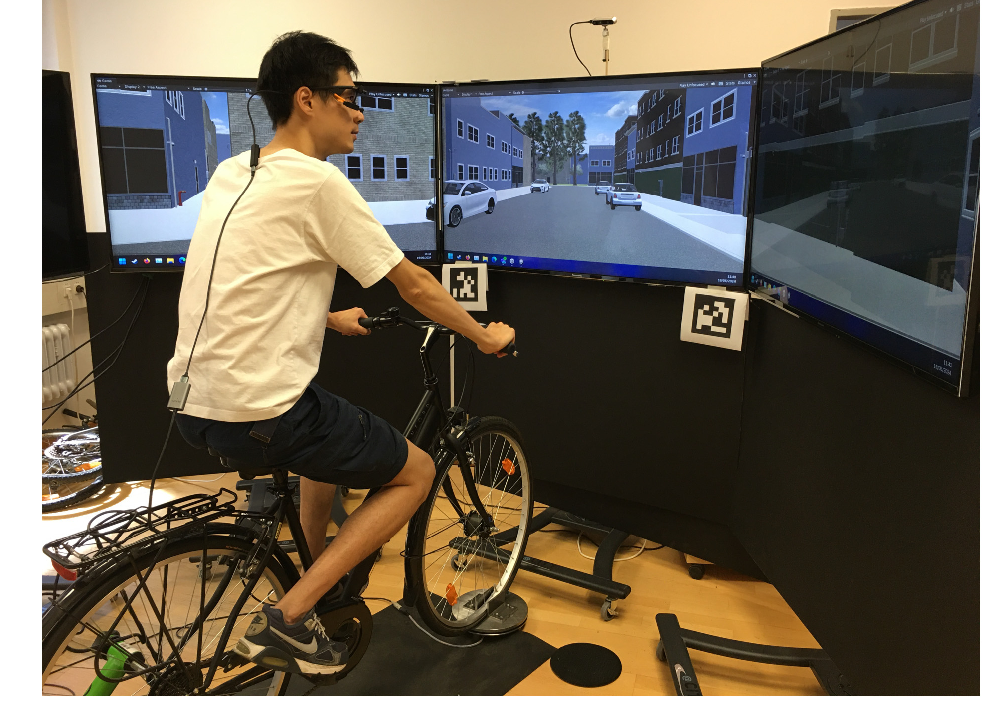
\includegraphics[width=0.72\linewidth]{fig1_simulator.pdf}
  \caption{The cycling simulator and eye-tracker used in the study.}
  \label{fig:simulator}
\end{figure}

% The two panels (a) shared path and (b) unsignalized intersection, with their
% sub-captions, are contained in the single graphic below. Use the subfigure
% environment instead if you want to re-label the panels yourself.
\begin{figure}[t]
  \centering
  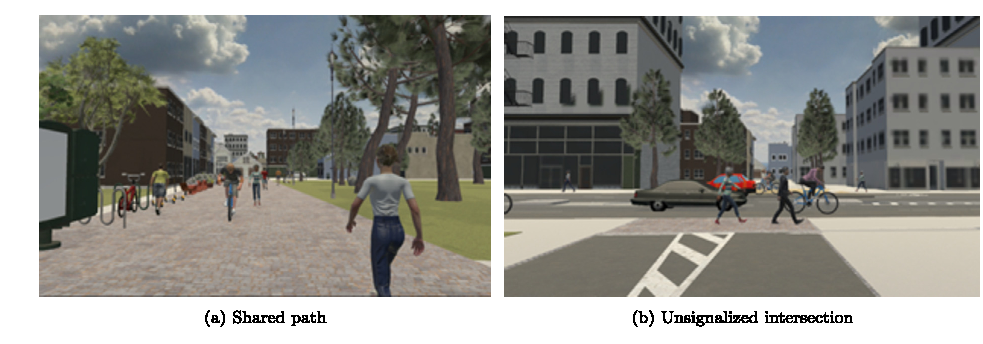
\includegraphics[width=\linewidth]{fig2_environments.pdf}
  \caption{Infrastructure in cycling simulator environment.}
  \label{fig:environments}
\end{figure}

\subsection{Experimental design}
The experiment consists of two environments; a shared path and an unsignalized
intersection, both shown in Fig.~\ref{fig:environments}. Their geometries are
shown in Fig.~\ref{fig:geometry}. In the shared path environment, pedestrians and
cyclists are expected to share the full width of the road without any priority
or dedicated areas to either pedestrians or cyclists. Even though some deviations
to speed and direction could be expected in real life, we assume that most users
of the shared path maintain their speed and direction to reduce complexity in the
setup of the experiment. At the unsignalized intersection the road users on the
minor road (including the participants) must give way to the crossing traffic on
the primary road. Therefore, in the experiment, all road users on the primary
road are programmed to maintain their speed and direction without yielding to the
participant. The software did not allow for any response in case of a collision
with other road users.

To understand how traffic and road conditions affect cyclist behavior and
subjective safety, we employ a full factorial design containing three attributes
with two levels for each environment, resulting in eight unique combinations of
attribute levels per environment (see Table~\ref{tab:design}). We define a
scenario as a unique combination of an attribute level and an environment.
Furthermore, we define a run as a pairing containing one shared path scenario and
one unsignalized intersection scenario. Eight of such runs (labeled 1--8) are
constructed. To reduce the learning effect, we swap the order of the environments
in four of the runs. Participants start with the shared path, followed by the
unsignalized intersection in runs 1, 2, 5, and 7, whereas the order is reversed
for the other four runs. As an example, Run 4 includes an unsignalized
intersection scenario characterized by high vehicle speed and low pedestrian and
bicycle flow (H/L/L), followed by a shared path scenario with high path width,
high pedestrian flow, and low bicycle flow (H/H/L).

Each participant completed eight runs. To minimize order effects and ensure that
participants did not ride in the same sequence from run 1 to 8, the order of the
runs was randomized into eight distinct courses using a Balanced Latin Square
Generator \citep{masson2024latin}. The total duration of the eight runs was
approximately 20 minutes.

\begin{figure}[t]
  \centering
  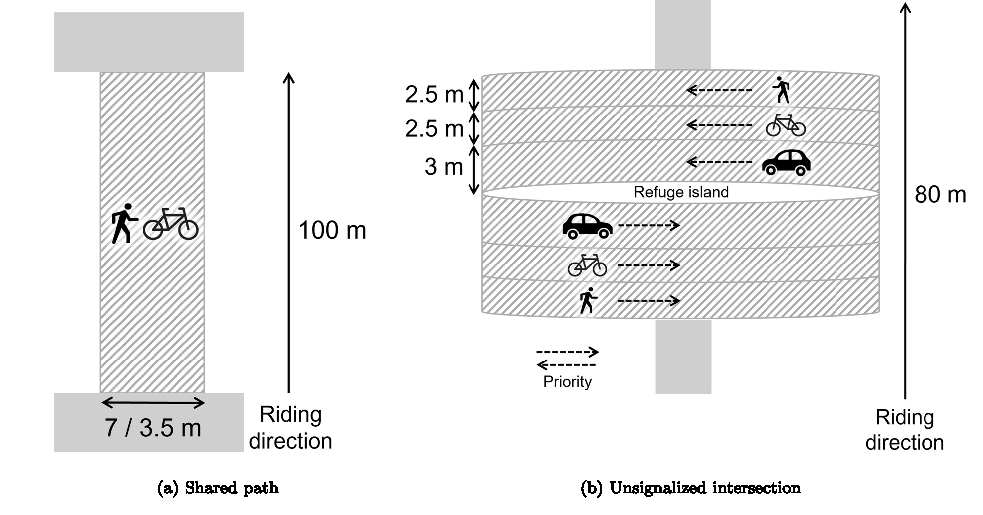
\includegraphics[width=0.88\linewidth]{fig3_geometry.pdf}
  \caption{Geometry of infrastructure environment.}
  \label{fig:geometry}
\end{figure}

\begin{table}[t]
  \centering
  \caption{Experimental design.}
  \label{tab:design}
  \small
  \begin{threeparttable}
  \begin{tabular}{@{}l l l cccccccc@{}}
    \toprule
    & & \multicolumn{1}{l}{Levels} & \multicolumn{8}{c}{Run}\\
    \cmidrule(l){4-11}
    \multirow{-2}{*}{Environment} & \multirow{-2}{*}{Attribute}
      & \multicolumn{1}{l}{Low (L) / High (H)}
      & 1 & 2 & 3\tnote{a} & 4\tnote{a} & 5 & 6\tnote{a} & 7 & 8\tnote{a}\\
    \midrule
    & Path width      & 3.5 / 7 [meters]              & H & L & L & H & L & H & H & L\\
    Shared path
    & Pedestrian flow & 250 / 500 [pedestrians/hour]  & H & L & H & H & L & L & L & H\\
    & Bicycle flow    & 250 / 500 [cyclists/hour]     & H & L & L & L & H & H & L & H\\
    \addlinespace[2pt]
    & Vehicle speed   & 20 / 40 [km/hour]             & L & L & H & H & H & L & L & H\\
    Unsignalized
    & Pedestrian flow & 500 / 1,000 [pedestrians/hour]& L & H & H & L & H & H & L & L\\
    intersection
    & Bicycle flow    & 350 / 700 [cyclists/hour]     & L & H & H & L & L & L & H & H\\
    \bottomrule
  \end{tabular}
  \begin{tablenotes}[flushleft]\footnotesize
    \item[a] The order of environment is reversed (i.e., unsignalized
      intersection before the shared path)
  \end{tablenotes}
  \end{threeparttable}
\end{table}

\subsubsection{Attribute levels}
The path width attributes are selected based on road design guidelines from the
Cycling Embassy of Denmark \citep{andersen2012collection} and the German
Research Association for Road and Traffic Engineering \citep{fgsv2010}, which
recommend a minimum width wider than 3 meters. Thus, we use a path width of 3.5
meters as the narrow attribute level. To assess how a wider path impacts
cyclists' behavior and psychological factors, we also include a 7-meter path,
which is also common in many European cities. In a cycling simulator environment
replicating the German context, \citet*{berghoefer2023prefer};
\citet{nazemi2021studying} chose 3.6 and 3.5 meters as the path width,
respectively.

The pedestrian flows are defined according to \citet{cyclenation2014} and
\citet{skoczynski2021analysis}, which suggest that the maximum pedestrian flow
on a shared path should be approximately 100 pedestrians per hour per meter of
width. Thus, we use 500 pedestrians per hour as the higher attribute level which
is equivalent to 71 and 142 pedestrians per hour per meter for wide and narrow
paths, respectively. To compare with a lower pedestrian flow and explore how the
amount of pedestrian flow influences cyclists' behavioral and psychological
factors, we selected 250 pedestrians per hour as the lower attribute level. For
the attribute levels of bicycle flow, we selected 250 and 500 cyclists per hour
as low and high levels, respectively. These represent reasonable flow rates on a
shared path and are distinct enough for meaningful comparison.

For the selection of attribute levels for the three attributes at the
unsignalized intersection, there are no strict criteria for vehicle speed and
pedestrian and bicycle flow \citep{andersen2012collection,jensen2012pedestrian}.
Therefore, the attribute levels were chosen by referring to the unsignalized
intersection with one of the highest near-crash-rate locations identified in
\citet{chou2024comparative} in Metropolitan Copenhagen, Denmark. We use 40 km/h
and 20 km/h for levels of high and low vehicle speed. Although the allowed speed
at this location is 50 km/h (similar to most urban roads in most EU countries
\citep{ec2024speed}), actual driving speeds are usually lower as drivers
anticipate crossing road users at the intersection and expect nearby traffic
signals. Therefore, we chose 40 km/h as the higher level for vehicle speed. We
conducted a pilot test to examine whether the lower level for vehicle speed
should be 30 km/h or 20 km/h, and eventually chose 20 km/h as participants
perceived a clearer distinction from 40 km/h at this speed. In the experiment,
scenarios with vehicle speeds of 40 km/h and 20 km/h feature the same number of
vehicles passing through the unsignalized intersection, leading to vehicle flows
of 500 and 1,000 vehicles per hour, respectively. The experiment also ensures
that participants have sufficient gaps to cross the unsignalized intersection in
both vehicle-speed scenarios. For pedestrian and bicycle flow, we selected 500
and 1,000 pedestrians per hour and 350 and 700 cyclists per hour as the high and
low attribute levels, ensuring they are reasonable and distinguishable.

\subsection{Indicators}
All behavioral and subjective safety indicators measured during the experiment
are shown in Table~\ref{tab:indicators}. In both infrastructure environments,
the participant's average speed is calculated by dividing the distance traveled
by the participant by the total crossing time, determined from the start and end
coordinates of infrastructure along with the corresponding time stamps. At
unsignalized intersections, the total crossing time includes cyclists
approaching the intersection, waiting time before starting to cross, and actual
crossing time.

\begin{table}[t]
  \centering
  \caption{Behavioral and subjective safety indicators.}
  \label{tab:indicators}
  \small
  \begin{tabular}{@{}p{0.24\linewidth} p{0.28\linewidth} p{0.40\linewidth}@{}}
    \toprule
    Environment & Variable & Measurement\\
    \midrule
    & Participant average speed [km/h]
      & Average speed passing through infrastructure\\
    \addlinespace[3pt]
    & Fixation rate [\%]
      & Percentage of total fixation duration on each road user to total
        crossing time\\
    \addlinespace[3pt]
    Shared path and
    & Perceived unsafety [5-point Likert]
      & \makecell[tl]{1: Very safe\\ 2: Somewhat safe\\
                      3: Neither safe nor unsafe\\ 4: Somewhat unsafe\\
                      5: Very unsafe}\\
    \addlinespace[3pt]
    Unsignalized intersection
    & Perceived stress [5-point Likert]
      & \makecell[tl]{1: No stress\\ 2: Low stress\\ 3: Moderate stress\\
                      4: High stress\\ 5: Very high stress}\\
    \bottomrule
  \end{tabular}
\end{table}

The fixation rate on road users in both environments is measured with an
eye-tracker. Fixation events on pedestrians, cyclists, or vehicles are manually
annotated. The rate for each road user is calculated by dividing the total
fixation events on them by the total crossing time in each environment.

Perceived unsafety and stress were assessed as subjective safety indicators
using a 5-point Likert scale in both infrastructure environments. Perceived
unsafety ranged from ``very safe'' to ``very unsafe,'' reflecting participants'
subjective sense of security while riding through each scenario. Perceived
stress ranged from ``no stress'' to ``very high stress,'' capturing participants'
emotional strain while riding through each scenario. Both indicators were
measured through post-run surveys conducted immediately after participants
completed each run (one for the shared path and one for the unsignalized
intersection).

\subsection{Experimental procedure}
The study was carried out in May and June of 2024. 50 participants were recruited
from various sources including the online platforms of the Technical University
of Munich, the mailing list of the Chair of Traffic Engineering and Control, and
the transportation-related institutions in the city of Munich (e.g., Municipality
and German National Cyclists' Association Munich branch). During the registration
process, participants were asked to complete a pre-study survey covering
demographic information, cycling habits, and their desired time for experiment
participation. During the experiment, participants were briefed about the study,
instructed on cycling simulator usage with a test ride, and asked to provide
informed consent before the experimental ride. Once participants had familiarized
themselves with the cycling simulator in the test ride, they started the
experiment. After each of the eight runs, participants had a short break and were
asked to rate their perceived unsafety and stress with a 5-point Likert scale
about the shared path and the unsignalized intersection scenarios. The average
completion time for the entire experiment was approximately one hour and
participants received a 15-euro shopping coupon as a reward.
Fig.~\ref{fig:dataflow} illustrates the overall methodological framework,
outlining the sequential steps of data acquisition, processing, and analysis in
the study.

\begin{figure}[t]
  \centering
  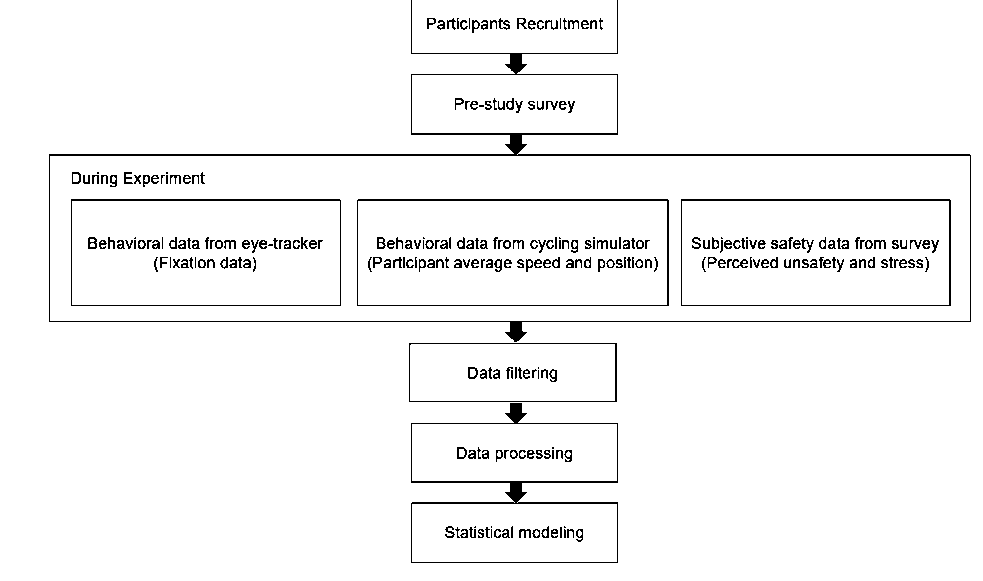
\includegraphics[width=0.9\linewidth]{fig4_dataflow.pdf}
  \caption{Data flow chart.}
  \label{fig:dataflow}
\end{figure}

\subsection{Statistical analysis}
After data was collected and processed, ordinary least square (OLS) regression
was used to explore how independent variables affect behavioral indicators, and
ordinal logistic regression was used to explore subjective safety indicators.

The specification of the OLS shown in formula~\eqref{eq:ols-speed} presenting
the relation between the behavior indicators, $Speed$, which denotes participant
average speed, and the participant $i$ in scenario $j$.
%
\begin{equation}\label{eq:ols-speed}
  \begin{aligned}
    Speed_{i,j} ={}& \alpha + \beta_1 Path\ width_j
                     + \beta_2 Pedestrian\ flow_j
                     + \beta_3 Bicycle\ flow_j\\
                   & + \beta_4 Path\ width_j \times Pedestrian\ flow_j\\
                   & + \beta_5 Path\ width_j \times Bicycle\ flow_j\\
                   & + \beta_6 Pedestrian\ flow_j \times Bicycle\ flow_j\\
                   & + \bm{\beta_7} \cdot
                       \bm{Individual\ dummies}_i + \epsilon .
  \end{aligned}
\end{equation}
%
Here $\alpha$ denotes the intercept of the model that is the expected mean when
all explanatory variables are zero. $Path\ width$ denotes the path width at the
shared path, while at the unsignalized intersection, this parameter is replaced
by $Vehicle\ speed$. $Pedestrian\ flow$ denotes pedestrian flow at both the
Shared path and the unsignalized intersection. Similarly, $Bicycle\ flow$
denotes bicycle flow at both infrastructure environments. All aforementioned
variables are dummies which are 1 when the high level is used, and 0 when the
low attribute level is used. $\bm{Individual\ dummies}$ denotes column
vectors of dummy variables including individual participants' characteristics.
$\bm{\beta_1}$ to $\bm{\beta_3}$ denotes coefficient of
explanatory variables. $\bm{\beta_4}$ to $\bm{\beta_6}$ denotes
coefficient of interaction terms between two explanatory variables.
$\bm{\beta_7}$ denotes vectors including coefficients of individual
dummy variables. $\epsilon$ denotes the error term indicating the effects of
factors not captured by the explanatory variables.

To examine the influence of behavioral and subjective indicators on fixation
patterns toward vehicles at unsignalized intersections, the OLS specification
presented in Equation~\eqref{eq:ols-fixation} was formulated.
%
\begin{equation}\label{eq:ols-fixation}
  \begin{aligned}
    Fixation\ on\ vehicles_{i,j} ={}&
        \alpha + \beta_1 Speed_j + \beta_2 Unsafety\\
      & + \beta_3 Vehicle\ speed_j + \beta_4 Pedestrian\ flow_j
        + \beta_5 Bicycle\ flow_j\\
      & + \beta_6 Vehicle\ speed_j \times Pedestrian\ flow_j\\
      & + \beta_7 Vehicle\ speed_j \times Bicycle\ flow_j\\
      & + \beta_8 Pedestrian\ flow_j \times Bicycle\ flow_j\\
      & + \bm{\beta_9} \cdot
          \bm{Individual\ dummies}_i + \epsilon .
  \end{aligned}
\end{equation}
%
In this context, $Fixation\ on\ vehicles$ refers to the fixation rate on
vehicles. It is important to note that $Unsafety$ is treated as a continuous
numerical variable rather than an ordinal one, as the differences between levels
of perceived unsafety are both meaningful and quantifiable. This treatment
supports the appropriate application of the OLS estimation.

The ordinal regression model is presented in equation~\eqref{eq:ordinal} below
presenting the relation between the subjective safety indicators, $Unsafety$,
which denotes perceived unsafety, and the participant $i$ in scenario $j$.
%
\begin{equation}\label{eq:ordinal}
  \begin{gathered}
    \mathrm{P}(Unsafety \leq n),\quad n = 1,2,3,4,5\\[4pt]
    \mathrm{Odds} = \frac{\mathrm{P}(Unsafety \leq n)}
                         {1-\mathrm{P}(Unsafety \leq n)}
                  = \frac{\mathrm{P}(Unsafety \leq n)}
                         {\mathrm{P}(Unsafety > n)}\\[4pt]
    \log(\mathrm{Odds}) = \log\!\left(
        \frac{\mathrm{P}(Unsafety \leq n)}{\mathrm{P}(Unsafety > n)}\right)
      = \mathrm{Logit}\bigl(\mathrm{P}(Unsafety \leq n)\bigr)\\[6pt]
    \begin{aligned}
      \mathrm{Logit}\bigl(\mathrm{P}(Unsafety_{i,j} \leq n)\bigr) ={}&
          \alpha_n + \beta_1 Speed_j\\
        & + \beta_2 Fixation\ rate_j\\
        & + \beta_3 Path\ width_j + \beta_4 Pedestrian\ flow_j
          + \beta_5 Bicycle\ flow_j\\
        & + \beta_6 Path\ width_j \times Pedestrian\ flow_j\\
        & + \beta_7 Path\ width_j \times Bicycle\ flow_j\\
        & + \beta_8 Pedestrian\ flow_j \times Bicycle\ flow_j\\
        & + \bm{\beta_9} \cdot
            \bm{Individual\ dummies}_i + \epsilon .
    \end{aligned}
  \end{gathered}
\end{equation}
%
Here $Unsafety$ has $n=5$ categories and $\mathrm{P}(Unsafety \leq n)$ represent
the cumulative probability of being in category $n$ or below, and it is modeled
across all threshold categories $n$. Odds represents the odds of being in a
lower category versus a higher category of the ordinal outcome. $\alpha_n$
denotes the intercept (also called thresholds or cut points) of the model that
distinguishes between the different levels of the ordinal dependent variable.

We included Participant average speed $Speed$ as an independent variable to
investigate whether behavioral and subjective indicators are interconnected. At
the unsignalized intersection, the $Path\ width$ is replaced by $Vehicle\ speed$.
We also included $Fixation$ as an independent variable since it is worth
investigating the relationship between perceived unsafety and the participant's
gazing behavior. The remaining independent variables and coefficients are as
same as the OLS model shown in formula~\eqref{eq:ols-speed}.

After estimating the models, the odds ratios (ORs) for each explanatory variable
were obtained by exponentiating the estimated coefficients (i.e.,
$e^{\bm{\beta_{1,2,\ldots 9}}}$). ORs provide a clear indication of how a
one-unit change in an independent variable influences the associated odds.

\subsection{Sample}
A total of 50 participants attended the experiment. One participant dropped out
due to motion sickness, and was discarded from the data. Participants were
selected based on the criteria of cycling at least once per month and having no
physical or psychological impairments. The eye movements of four participants
could not be detected, likely due to reflections from glasses or makeup.
Therefore, eye-tracker fixation data is only available for 45 participants. The
49 participants who completed the experiment included 16 (32.7\%) females and 33
(67.3\%) males. Their age composition is 20-29 (11, 22.4\%), 30-39 (11, 22.4\%),
40-49 (12, 24.5\%), 50-59 (10, 20.4\%), 60-69 (3, 6.1\%), and 70-79 (2, 4.1\%).
For their cycling frequency in a recent year, 30 (61.2\%) ride almost every day,
10 (20.4\%) ride every two to three days in a week, 5 (10.2\%) ride once a week,
1 (2.0\%) rides once every two weeks, and 3 (6.1\%) ride once a month. For their
trip purpose, 25 (51.0\%) ride for work, 2 (4.1\%) ride for school, 7 (14.3\%)
ride for leisure, 6 (12.2\%) ride for errand, 3 (6.1\%) ride for social
activities, and 6 (12.2\%) ride for other purposes.

%=====================================================================
\section{Results}\label{sec:results}
%=====================================================================
This section will present the descriptive analysis of the data collected from
the experiment and the outcomes of the model estimation results. In the model
estimation results, all parameters are significant at the 5\% level. In~\ref{app:allvariables} we
present the models with all tested
attributes. It is important to mention that all models account for individual
participants' characteristics as dummy variables (i.e.,
$\bm{Individual\ dummies_i}$ in formula~\eqref{eq:ols-speed}), but these
are not included in the tables since they are not the focus of our analysis.

\subsection{Analysis of cyclists in behavior in the shared path scenario}

\indicatorhead{Participant average speed}
Fig.~\ref{fig:speed-shared} shows boxplots of participant average speeds across
the eight shared path scenarios (for more information on the scenarios, we refer
to Table~\ref{tab:design}). As seen in the figure, the width of the shared path
seems to affect speed, as the four ``wide'' scenarios also have the highest
speed. When both the bicycle and pedestrian flow is low, the participant's
average speed is higher than in all other combinations of the flow attributes in
the narrow and wide scenarios.

For the model estimating participant average speed on the shared path shown in
Table~\ref{tab:ols-shared}, all three attributes and the interaction between
pedestrian flow and bicycle flow are significant. The average speed rises the
most (by 2.8 km/hour) when the path width expands from narrow (3.5 meters) to
wide (7 meters). The average speed decreases by 1.8 km/hour when pedestrian flow
rises from low (250 pedestrians/hour) to high (500 pedestrians/hour). Similarly,
the average speed decreases by 1.5 km/hour when bicycle flow rises from low (250
cyclists/hour) to high (500 cyclists/hour). When both pedestrian and bicycle
flows increase from low to high, the average speed decreases by 1.4 km/hour due
to the interaction effect.

\begin{figure}[t]
  \centering
  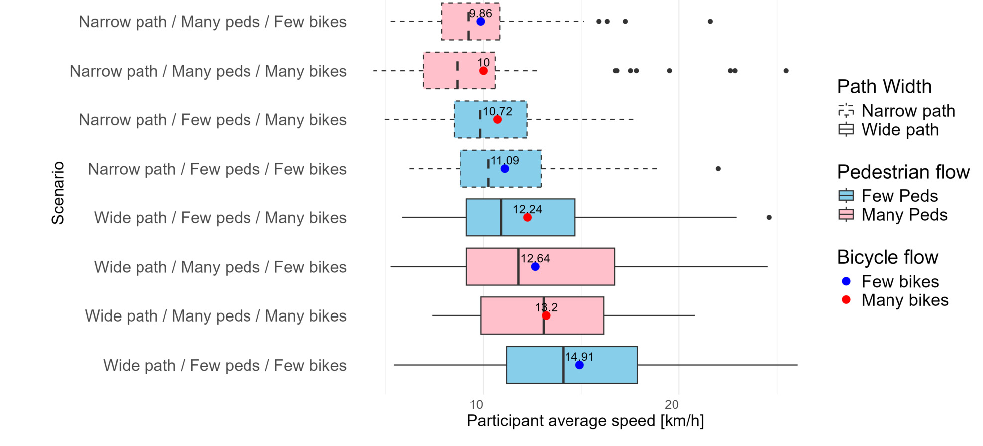
\includegraphics[width=\linewidth]{fig5_speed_shared.pdf}
  \caption{Participant average speed in eight scenarios (combination of
    environment and variable values) at the shared path environment. Dots
    indicate the mean value.}
  \label{fig:speed-shared}
\end{figure}

\begin{table}[t]
  \centering
  \caption{Model estimation results for participant average speed at the shared
    path.}
  \label{tab:ols-shared}
  \small
  \begin{threeparttable}
  \begin{tabular}{@{}l r r r l@{}}
    \toprule
    Variables & Coefficient & Std. error & t-value & p-value\\
    \midrule
    \multicolumn{5}{c}{Participant average speed [km/hour]}\\
    \addlinespace[2pt]
    Intercept                                       & 17.159 & 1.185 & 14.483 & \pvl\ ***\\
    Path width high                                 &  2.832 & 0.325 &  8.702 & \pvl\ ***\\
    Pedestrian flow high                            & -1.751 & 0.460 & -3.803 & 0.001 ***\\
    Bicycle flow high                               & -1.521 & 0.460 & -3.304 & 0.001 ***\\
    Pedestrian flow high $\times$ Bicycle flow high &  1.870 & 0.651 &  2.873 & 0.004 ***\\
    \midrule
    \multicolumn{2}{@{}l}{Adjusted R-squared} & \multicolumn{3}{l}{0.485}\\
    \bottomrule
  \end{tabular}
  \begin{tablenotes}[flushleft]\footnotesize
    \item \sigstars
  \end{tablenotes}
  \end{threeparttable}
\end{table}

\indicatorhead{Perceived unsafety}
Fig.~\ref{fig:unsafety-shared} shows boxplots of participants indicated
subjective safety across the eight shared path scenarios. We only show the
results of perceived unsafety since the correlation between perceived unsafety
and stress is very high (74\% in both environments). The corresponding figures
for perceived stress are in~\ref{app:unsafetystress}.

Participants riding in narrow shared-path scenarios have higher perceived
unsafety than those riding in wide-shared-path scenarios. Moreover, participants
riding in narrow shared-path scenarios felt more unsafe when pedestrian and
bicycle flow increased from low to high simultaneously.

For the model estimating perceived unsafety on the shared path shown in
Table~\ref{tab:ord-shared}, participant average speed, all three attributes, and
interactions between path width and bicycle flow are significant. Participant
average speed and path width have odds ratios lower than 1, meaning that faster
average speed and wider paths are associated with a lower level of perceived
unsafety. The odds of perceiving a higher level of unsafety decrease by about
54.2\% (i.e., 1 - 0.458) when increasing the width from narrow to wide. For
comparison, a similar effect can be found when increasing the speed by 6.5 km/h
(i.e., 1 - $(0.887)^{6.5}$ = 0.54).

\begin{figure}[t]
  \centering
  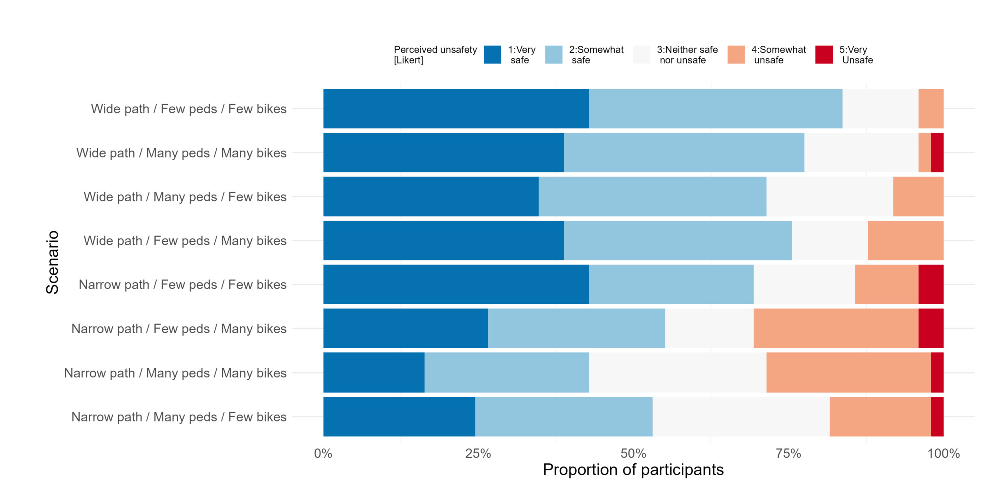
\includegraphics[width=\linewidth]{fig6_unsafety_shared.pdf}
  \caption{Perceived unsafety in eight scenarios at the shared path environment.}
  \label{fig:unsafety-shared}
\end{figure}

\begin{table}[t]
  \centering
  \caption{Model estimation results for perceived unsafety at the shared path.}
  \label{tab:ord-shared}
  \small
  \begin{threeparttable}
  \begin{tabular}{@{}l r r r l@{}}
    \toprule
    Variables & Odds ratio & Std. error & t-value & p-value\\
    \midrule
    \multicolumn{2}{@{}l}{Intercepts (Thresholds)}
      & \multicolumn{3}{l}{Perceived unsafety [Likert]}\\
    \addlinespace[2pt]
    Perceived unsafety 1 vs 2 (or higher)              &  0.019 & 0.549 & -7.209 & \pvl\ ***\\
    Perceived unsafety 2 (or lower) vs 3 (or higher)   &  0.295 & 0.502 & -2.431 & 0.015 *\\
    Perceived unsafety 3 (or lower) vs 4 (or higher)   &  2.368 & 0.507 &  1.702 & 0.089\\
    Perceived unsafety 4 (or lower) vs 5               & 99.086 & 0.722 &  6.363 & \pvl\ ***\\
    \addlinespace[2pt]
    Participant average speed high                     &  0.887 & 0.033 & -3.672 & \pvl\ ***\\
    Path width high                                    &  0.458 & 0.319 & -2.447 & 0.014 *\\
    Pedestrian flow high                               &  1.728 & 0.216 &  2.532 & 0.011 *\\
    Bicycle flow high                                  &  3.145 & 0.304 &  3.768 & \pvl\ ***\\
    Path width high $\times$ Bicycle flow high         &  0.326 & 0.431 & -2.600 & 0.009 **\\
    \midrule
    \multicolumn{2}{@{}l}{Akaike information criterion (AIC)}
      & \multicolumn{3}{l}{791.16}\\
    \bottomrule
  \end{tabular}
  \begin{tablenotes}[flushleft]\footnotesize
    \item \sigstars
  \end{tablenotes}
  \end{threeparttable}
\end{table}

Pedestrian and bicycle flow have odds ratios larger than 1, meaning that an
increase from low to high in both cases is associated with a higher likelihood of
perceived unsafety. The odds of high-level perceived unsafety increase by about
72.8\% and 214.5\%, respectively. When both path width and bicycle flow increase
from low to high, the perceived unsafety does not change much compared to
low-path-width and high-bicycle-flow scenarios due to the interaction effect.
This indicates that in the low path-width scenario, the bicycle flow does not
play an important role.

\subsection{Unsignalized intersection}

\indicatorhead{Participant average speed}
Fig.~\ref{fig:speed-unsig} shows that at unsignalized intersections, participant
average speed is higher when the vehicle speed is low compared to when the
vehicle's speed is high. Among the slow-vehicle scenarios, the participant
average speed is lower when pedestrian flow is high compared to low pedestrian
flow.

For the model estimating participant average speed at the unsignalized
intersection shown in Table~\ref{tab:ols-unsig}, vehicle speed, pedestrian flow,
and their interaction are significant. The average speed reduces by 6.7 km/hour
when the vehicle speed increases from low (20 km/hour) to high (40 km/hour), and
it reduces by 3.5 km/hour when the pedestrian flow increases from low (500
pedestrians/hour) to high (1000 pedestrians/hour). When both vehicle speed and
pedestrian flow increase from low to high, the average speed reduces by 5.7
km/hour.

\begin{figure}[t]
  \centering
  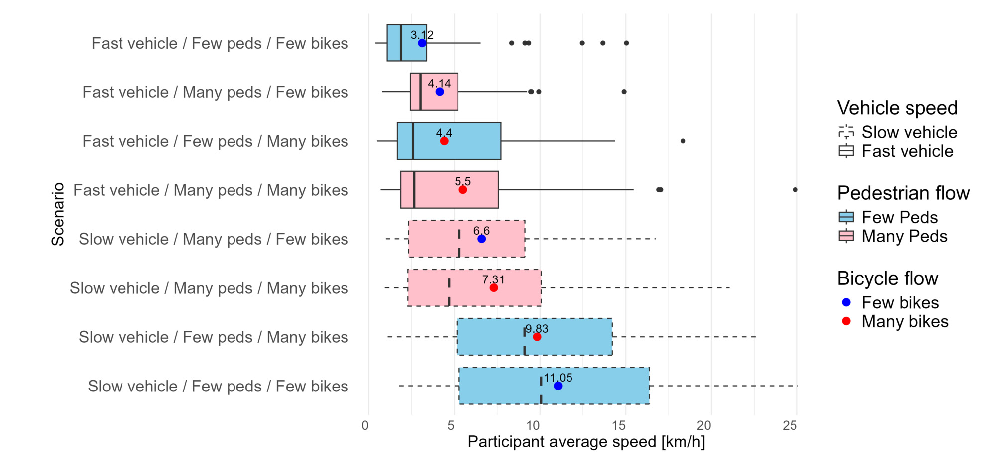
\includegraphics[width=\linewidth]{fig7_speed_unsig.pdf}
  \caption{Participant average speed in eight scenarios at unsignalized
    intersection environment. Dots indicate the mean value.}
  \label{fig:speed-unsig}
\end{figure}

\begin{table}[t]
  \centering
  \caption{Model estimation results for participant average speed at the
    unsignalized intersection.}
  \label{tab:ols-unsig}
  \small
  \begin{threeparttable}
  \begin{tabular}{@{}l r r r l@{}}
    \toprule
    Variables & Coefficient & Std. error & t-value & p-value\\
    \midrule
    \multicolumn{5}{c}{Participant average speed [km/hour]}\\
    \addlinespace[2pt]
    Intercept                                     &  15.378 & 1.598 &   9.626 & \pvl\ ***\\
    Vehicle speed high                            &  -6.678 & 0.621 & -10.752 & \pvl\ ***\\
    Pedestrian flow high                          &  -3.486 & 0.621 &  -5.612 & \pvl\ ***\\
    Vehicle speed high $\times$ Pedestrian flow high &   4.547 & 0.878 &   5.177 & \pvl\ ***\\
    \midrule
    \multicolumn{2}{@{}l}{Adjusted R-squared} & \multicolumn{3}{l}{0.390}\\
    \bottomrule
  \end{tabular}
  \begin{tablenotes}[flushleft]\footnotesize
    \item \sigstars
  \end{tablenotes}
  \end{threeparttable}
\end{table}

\indicatorhead{Perceived unsafety}
The perceived unsafety at the unsignalized intersection, shown in
Fig.~\ref{fig:unsafety-unsig}, indicates that participants had higher perceived
unsafety when they rode in high-vehicle-speed scenarios.

For the model estimating perceived unsafety at the unsignalized intersection
shown in Table~\ref{tab:ord-unsig}, participant average speed, vehicle speed,
bicycle flow, and fixation on vehicles are significant. Participant average
speed has an odds ratio lower than 1, meaning that for every kilometer per hour
increase in average speed, the odds of perceiving higher levels of unsafety
decrease by 21.4\%. Vehicle speed, bicycle flow, and fixation on vehicles have
odds ratios larger than 1, meaning that for every unit increase, the odds of
perceiving higher levels of unsafety increase by 264.3\%, 82.8\%, and 6\%,
respectively, showcasing that vehicle speed by far is the most influential
factor.

\begin{figure}[t]
  \centering
  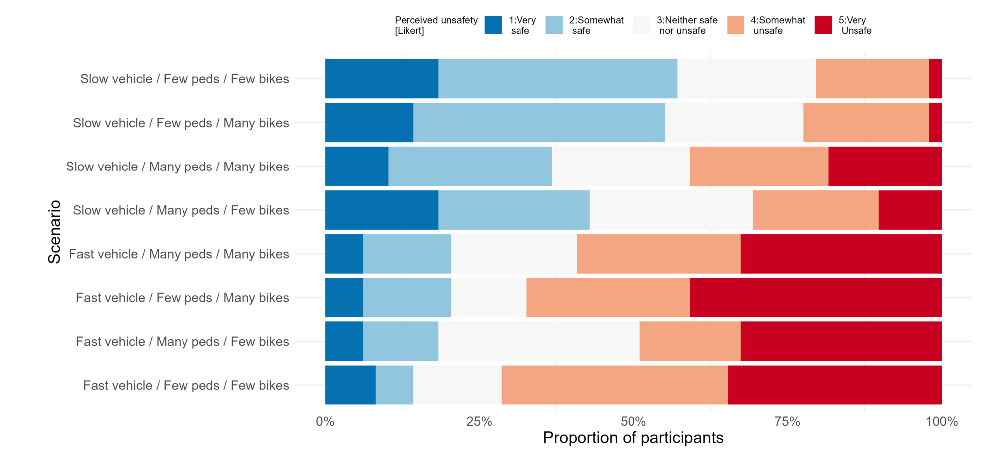
\includegraphics[width=\linewidth]{fig8_unsafety_unsig.pdf}
  \caption{Perceived unsafety in eight scenarios at the unsignalized
    intersection environment.}
  \label{fig:unsafety-unsig}
\end{figure}

\begin{table}[t]
  \centering
  \caption{Model estimation results for perceived unsafety at the unsignalized
    intersection.}
  \label{tab:ord-unsig}
  \small
  \begin{threeparttable}
  \begin{tabular}{@{}l r r r l@{}}
    \toprule
    Variables & Odds ratio & Std. error & t-value & p-value\\
    \midrule
    \multicolumn{2}{@{}l}{Intercepts (Thresholds)}
      & \multicolumn{3}{l}{Perceived unsafety [Likert]}\\
    \addlinespace[2pt]
    Perceived unsafety 1 vs 2 (or higher)            & 0.004 & 0.813 & -6.886 & \pvl\ ***\\
    Perceived unsafety 2 (or lower) vs 3 (or higher) & 0.063 & 0.746 & -3.707 & \pvl\ ***\\
    Perceived unsafety 3 (or lower) vs 4 (or higher) & 0.453 & 0.731 & -1.084 & 0.278\\
    Perceived unsafety 4 (or lower) vs 5             & 3.244 & 0.736 &  1.598 & 0.110\\
    \addlinespace[2pt]
    Participant average speed high                   & 0.786 & 0.030 & -8.130 & \pvl\ ***\\
    Vehicle speed high                               & 3.643 & 0.251 &  5.155 & \pvl\ ***\\
    Bicycle flow high                                & 1.828 & 0.217 &  2.775 & 0.006 **\\
    Fixation on vehicles (\%)                        & 1.060 & 0.019 &  3.139 & 0.002 ***\\
    \midrule
    \multicolumn{2}{@{}l}{Akaike information criterion (AIC)}
      & \multicolumn{3}{l}{831.19}\\
    \bottomrule
  \end{tabular}
  \begin{tablenotes}[flushleft]\footnotesize
    \item \sigstars
  \end{tablenotes}
  \end{threeparttable}
\end{table}

\indicatorhead{Fixation on vehicles}
For the model estimating fixation on vehicles at the unsignalized intersection
shown in Table~\ref{tab:ols-fixation}, participant average speed, vehicle speed,
and pedestrian flow are significant. A drop in average participant speed of 1
kilometer per hour is associated with a 0.3\% increase in fixation on vehicles.
Fixation is also reduced by 2.2\% when pedestrian flow increases from low to
high. The fixation on vehicles rises by 3.5\% when vehicle speed rises from low
to high.

\begin{table}[t]
  \centering
  \caption{Model estimation results for fixation on vehicles at the unsignalized
    intersection.}
  \label{tab:ols-fixation}
  \small
  \begin{threeparttable}
  \begin{tabular}{@{}l r r r l@{}}
    \toprule
    Variables & Coefficient & Std. error & t-value & p-value\\
    \midrule
    \multicolumn{5}{c}{Fixation on vehicles [\%]}\\
    \addlinespace[2pt]
    Intercept                      &  9.658 & 2.644 &  3.653 & \pvl\ ***\\
    Participant average speed high & -0.262 & 0.083 & -3.165 & 0.002 ***\\
    Vehicle speed high             &  3.457 & 0.788 &  4.388 & \pvl\ ***\\
    Pedestrian flow high           & -2.176 & 0.703 & -3.095 & 0.002 ***\\
    \midrule
    \multicolumn{2}{@{}l}{Adjusted R-squared} & \multicolumn{3}{l}{0.578}\\
    \bottomrule
  \end{tabular}
  \begin{tablenotes}[flushleft]\footnotesize
    \item \sigstars
  \end{tablenotes}
  \end{threeparttable}
\end{table}

%=====================================================================
\section{Discussion}\label{sec:discussion}
%=====================================================================
Our findings provide important evidence on how the width of a shared path
influences cyclists' perceived safety and riding behavior. In line with
\citet{gkekas2020perceived} and \citet{hummer2005user}, we observe that cyclists
feel significantly safer when path width is increased. One likely reason is the
reduction in conflicts among users, as also suggested by
\citet{boufous2018impact}, who found that cyclists tend to ride faster on wider
paths, a pattern confirmed in our study. Quantitatively, our results suggest
that widening a 100-meter-long shared path used by 5,000 cyclists daily from 3.5
to 7 meters could result in approximately 2,700 cyclists reporting a lower
perceived unsafety category. In addition, every cyclist would, on average,
increase their speed on this stretch by 2.8 km/h.

At unsignalized intersections, our results show that cyclists feel significantly
less safe when the speed of approaching vehicles is higher. This finding is
consistent with \citet{beura2021unsignalized} and \citet{jensen2012pedestrian},
who suggest that higher vehicle speeds and increased traffic flow contribute to a
reduced sense of safety among vulnerable road users. Moreover, we observe that
cyclists' average speed decrease as they are forced to wait longer for acceptable
gaps in traffic, leading to increased overall travel times. This highlights a
clear trade-off between car drivers' mobility and cyclists' mobility: while
higher vehicle speeds may benefit drivers by reducing their travel times, they
simultaneously reduce perceived safety and increase delays for cyclists.
According to our results, at an unsignalized intersection with similar geometry
to our experimental setup, reducing vehicle speed from 40 km/h to 20 km/h would
lead to a 12 km/h increase in cyclists' average speed while approaching,
crossing, and exiting the intersection. These findings underscore an important
and often overlooked point in transport planning: cyclists' mobility is rarely
integrated into traditional transport planning methods, which primarily focus on
minimizing travel time for motorized vehicles and consider safety for active
travelers. Our results emphasize the need for a more balanced approach that
recognizes cyclists not merely as safety concerns but as legitimate road users
with mobility needs. By explicitly incorporating cyclists' travel time and
perceived safety into planning and modeling frameworks, policymakers and
engineers can design intersections and networks that support equitable and
sustainable transport systems.

In both environments, we found a similar tendency in the relationship between
flows of other bicyclists and pedestrians and how this affects both the cyclists'
perceived unsafety and their average speed. Generally, cyclists felt less safe as
pedestrian and bicycle traffic increased at shared paths and unsignalized
intersections. Previous studies for shared paths
\citep{berghoefer2023prefer,gkekas2020perceived} have found similar patterns.
Interestingly, bicycle flow had nearly twice the impact on perceived unsafety
than pedestrian flow at shared paths, likely because cyclists move faster and
pose a greater risk of severe crashes. We also find that cyclists perceive a
wider shared path with higher bicycle flow as safer than a narrower path with
lower bicycle flow, even when both scenarios have the same traffic density (road
users per area). This perception may stem from the broader visual space, which
gives cyclists a sense of having more space to maneuver and reduces the perceived
risk of collisions with other bicycles. Finally, we found a negative correlation
between cyclists' perceived unsafety and participant average speed in both
environments, largely due to common contributing factors affecting both
indicators. This outcome is intuitive, as cyclists forced to ride slower tend to
feel less safe. Improving cyclists' mobility can therefore enhance their
perceived safety and vice versa.

These findings underscore the need for planners, architects, and engineers to go
beyond observed safety, aesthetic, and experiential considerations when designing
cycling infrastructure. By incorporating quantitative evidence on mobility and
perceived safety and behavior from studies like ours, they can better address
users' actual needs and create environments that encourage cycling. Prioritizing
wider paths can thus contribute to both improved subjective safety and more
efficient flow, ultimately supporting broader policy goals of promoting active
and sustainable transportation.

Finally, while our study highlights the importance of improving bicycle traffic
flow and reducing perceived unsafety, these goals should never come at the
expense of actual safety. Our results also provide new insights into how
cyclists' attention to motorized traffic is shaped by various factors. Cyclists
riding at higher speeds tend to focus less on vehicles, potentially prioritizing
their own movement over monitoring traffic. In contrast, higher vehicle speeds
increase cyclists' fixation on cars, reflecting a heightened need for caution.
Interestingly, higher pedestrian flow appears to draw cyclists' attention away
from vehicles, likely because they must navigate around other vulnerable road
users. Determining the design of an intersection should thus depend on multiple
contextual factors, including the dominant type of cyclists (e.g., commuters
versus leisure riders), their typical speeds, and the level of pedestrian
activity. By accounting for these elements and integrating both perceived and
actual safety considerations, planners and engineers can better create
intersections that accommodate diverse user needs.

\subsection{Limitation and future research}
Although we were able to quantify and confirm our hypotheses using the cycling
simulator experiments, a few limitations are worth mentioning. In our setup,
participants lack a 360-degree virtual environment for full immersion, and the
static cycling simulator prevents them from leaning while steering. These
technical limitations make the simulation less realistic. Furthermore, in the
simulation environments, the visualized pedestrians and cyclists can only travel
straight and cannot interact with participants. This may have led to behaviors
and subjective safety assessments differing from those typically present in real
life. At most unsignalized intersections in cities with high cycling contexts,
vehicles often yield to cyclists, even when they have the right of way. Some
participants expected this yielding behavior, which influenced their actions,
despite being informed before the experiment that vehicles had priority and would
not yield. Similar experiences are described in \citet*{berghoefer2023prefer}.

Future research could enhance realism by improving the technical setups and user
interactions in the simulation environment. Additionally, incorporating
individual characteristics such as their riding styles, riding experience, and
safety awareness could help explore how personal features influence cycling
behaviors and subjective safety. Our experiment can also be replicated with
different design configurations of shared paths and unsignalized intersections to
gain more comprehensive insights into cyclists' behavior and perceived safety.
Such research would help improve the understanding of cyclist safety, mobility,
and riding experiences across these two types of infrastructure.

Finally, a few insights from our modeling process are worth highlighting. We
explored the relationship between fixation on cars and cyclists' perceived
unsafety in both the model for perceived unsafety and the model for fixation
time. However, we did not find a plausible result that combined a clear direction
and statistical significance in both models. While it would seem most intuitive
that cyclists who feel less safe would fixate longer on cars, this effect was not
significant in the model with fixation time as the dependent variable.
Conversely, we did find a significant parameter for fixation time in the model
describing perceived unsafety, indicating that cyclists who fixate longer on cars
tend to report feeling more unsafe. This relationship is likely correlational
rather than causal, and the overall model results do not provide a consistent or
robust interpretation. Therefore, we chose not to include this relationship
explicitly in our final models. Previous studies provide mixed evidence on this
topic: \citet{mohammadi2024understanding} suggest that longer fixation on
vehicles is associated with lower perceived safety because cyclists are uncertain
about drivers' intentions to yield, making them feel more cautious. In contrast,
\citet{stulpnagel2020gaze} found that a higher perceived hazard can lead to
shorter fixation times, as cyclists may shift their gaze to scan the environment
more broadly.

%=====================================================================
\section{Conclusion}\label{sec:conclusion}
%=====================================================================
This study uses a cycling simulator to examine and quantify how path widths on
shared paths, vehicle speeds at unsignalized intersections, and pedestrian and
bicycle flow in both environments affect cyclist behavior and subjective safety.
The experiment employed a full factorial design, allowing participants to
experience environments with all possible combinations of the three attributes.
Behavioral and subjective safety data collected from participants were then
analyzed using a statistical modeling approach. We found that participant average
speed and perceived unsafety are significantly associated with all measured
attributes and quantified each effect.

The study provides new evidence on how shared path width, vehicle speed at
intersections, and surrounding traffic flows influence cyclists' perceived safety
and riding behavior. Our findings confirm that wider paths significantly enhance
cyclists' feelings of safety and promote higher cycling speeds, while higher
vehicle speeds at unsignalized intersections reduce cyclists' sense of safety and
slow their movement. These results emphasize the trade-off between motorized and
non-motorized mobility and highlight the importance of designing infrastructure
that prioritizes both perceived and actual safety for cyclists.

We also show that cyclists' perceptions are strongly affected by interactions
with other road users. In particular, higher flows of pedestrians and cyclists
generally increase perceived unsafety, yet a wider path with higher bicycle flow
can still be perceived as safer due to increased maneuvering space. Furthermore,
our analysis of gaze behavior suggests that cyclists' attention to vehicles
depends on their own riding speed, vehicle speed, and pedestrian density,
underlining the importance of considering user context when designing
intersections and shared spaces.

Overall, our findings contribute to a growing body of evidence supporting the
design of cycling environments that not only improve safety but also promote
greater comfort and efficiency for cyclists. By integrating these insights into
transport models and urban planning, cities can better support active travel and
create more sustainable, user-centered transport systems.

%=====================================================================
\section*{CRediT authorship contribution statement}
%=====================================================================
\textbf{Kuan-Yeh Chou:} Writing -- review \& editing, Writing -- original draft,
Visualization, Validation, Software, Resources, Methodology, Investigation,
Formal analysis, Data curation, Conceptualization. \textbf{Mads Paulsen:}
Writing -- review \& editing, Supervision, Methodology, Conceptualization.
\textbf{Mette Møller:} Writing -- review \& editing, Supervision, Methodology,
Conceptualization. \textbf{Anders Fjendbo Jensen:} Writing -- review \& editing,
Supervision, Methodology, Conceptualization.

%=====================================================================
\section*{Data availability}
%=====================================================================
The data that has been used is confidential.

%=====================================================================
\appendix
%=====================================================================
%  Appendices A-C
%
%  The published article numbers appendix tables and figures continuously
%  with the main text (Table 7 is followed by Table A.8; Fig. 8 by
%  Fig. B.9). The counters are therefore set explicitly below instead of
%  being reset at each appendix section.
%=====================================================================

% Cells of the literature-review tables are set ragged right, as in the
% published article.
\newcolumntype{R}[1]{>{\raggedright\arraybackslash}p{#1}}

% Appendix tables/figures carry the appendix letter as a prefix: "A.8", not
% "Appendix A.8" (\thesection spells out "Appendix A" in elsarticle).
\renewcommand{\thetable}{\Alph{section}.\arabic{table}}
\renewcommand{\thefigure}{\Alph{section}.\arabic{figure}}

%---------------------------------------------------------------------
\section{Literature review}\label{app:literature}
%---------------------------------------------------------------------
\setcounter{table}{7}   % next table becomes A.8

See Tables~\ref{tab:litreview1} and~\ref{tab:litreview2}.

{\scriptsize
\setlength{\tabcolsep}{3pt}
\renewcommand{\arraystretch}{1.05}
\begin{longtable}{@{}
    R{0.085\linewidth}
    R{0.075\linewidth}
    R{0.135\linewidth}
    R{0.095\linewidth}
    R{0.145\linewidth}
    R{0.095\linewidth}
    R{0.085\linewidth}
    R{0.185\linewidth}@{}}
  \caption{Summary of studies exploring cyclists' behavior and subjective safety
    at shared paths (Part 1).}\label{tab:litreview1}\\
  \toprule
  Study & Study area & Objective & Data collection method & Attributes
    & Behavior Indicators & Subjective Indicators & Findings\\
  \midrule
  \endfirsthead
  \multicolumn{8}{@{}l}{\textit{Table \thetable\ (continued)}}\\
  \toprule
  Study & Study area & Objective & Data collection method & Attributes
    & Behavior Indicators & Subjective Indicators & Findings\\
  \midrule
  \endhead
  \bottomrule
  \endlastfoot

  \multicolumn{8}{@{}l}{\textbf{Shared path}}\\
  \addlinespace[2pt]

  \citet{kazemzadeh2024forwhom}
    & Lund, Sweden
    & Explore cyclists' comfort during interactions in shared spaces,
      considering demographic heterogeneity
    & Intercept survey (594 cyclists)
    & 1. Cyclist demographics (age/gender/education)
      2. Cycling experience
      3. Interaction type (passing/meeting)
    &
    & Comfort
    & 1. Female cyclists, older adults, and less experienced cyclists generally
      report lower comfort in shared spaces
      2. Significant demographic differences affect comfort perception,
      highlighting the need for targeted infrastructure improvements.\\
  \addlinespace[4pt]

  \citet*{vonstulpnagel2024matter}
    & Berlin, Germany
    & Explore how environmental and demographic factors affect cyclists'
      perceived safety
    & Survey (21,500 participants)
    & 1. Buffer type between cycling and pedestrian lane
      (None/Greens/Cobbled)
      2. Sidewalk usage (Free/Cafes/shops)
    &
    & Perceived safety
    & Cyclists feel safe on sidewalks shared with pedestrians, at the expense of
      pedestrians' subjective safety\\
  \addlinespace[4pt]

  \citet*{berghoefer2023prefer}
    & Braun\-schweig (Campus), Germany
    & Explore factors affecting cyclists' infrastructure preferences and
      subjective safety
    & Cycling simulator (39 participants)
    & Advisory lane/Cycle path/Footpath:
      1. Pedestrian volume (5/25 [pedestrians])
      2. Vehicle volume (200/1000 [veh/h])
      Street/Multi-use path:
      1. Pedestrian volume (5/25 [pedestrians])
      2. Vehicle volume (100/400 [veh/h])
    &
    & 1. Mental Comfort
      2. Interaction
      3. Environment
      4. Ease of Use
      5. Physical Comfort
    & 1. Cycle paths that are separated from other road users were most
      preferred, while crowded footpaths and uphill segments were least
      preferred
      2. Cyclists riding on paths/lanes involving pedestrians felt less safe and
      comfortable when pedestrian volume was higher.\\
  \addlinespace[4pt]

  \citet{batista2023exploring}
    & Braun\-schweig, Germany
    & Explore factors affecting pedestrians' and cyclists' infrastructure
      preferences
    & Survey (408 participants)
    & 1. Space configuration (central placement of design
      elements/segregation types)
      2. Design elements (benches/fountains/bol\-lards/play elements)
      3. Presence of motor vehicles
    & 1. Crossing path choice
      2. Interaction behaviors
    & 1. Comfort
      2. Enjoyment level
      3. Preference for design attributes
    & 1. Both pedestrians and cyclists favor centrally located design elements
      and protective barriers.
      2. Motor vehicles are perceived negatively by both pedestrians and
      cyclists.
      3. Effective shared space designs incorporate integration, placemaking,
      and informal segregation.\\
  \addlinespace[4pt]

  \citet{zhang2023space}
    & Global (Systematic Review)
    & Explore interactions and safety between pedestrians and micro-mobility
      vehicles (MMVs) in shared spaces
    & Systematic literature review (87 publications)
    & 1. Infrastructure features
      2. Road user characteristics
      3. Operation condition
    & 1. Swerving
      2. Passing
      3. Overtaking
      4. Lateral displacement
    & 1. Perceived safety
      2. Comfort level
      3. Attitudes toward pedestrians
    & Key factors include sufficient infrastructure width, clear regulations,
      and speed management. Effective solutions include user education and
      infrastructure improvements.\\
  \addlinespace[4pt]

  \citet{pashkevich2022visual}
    & Kraków, Poland
    & Explore visual attention and speeds of pedestrians, cyclists, and electric
      scooter (ES) riders
    & Field experiment with eye tracker (12 participants)
    & 1. Visual attention distribution (roadway/roadside/all three road users)
      2. Speeds and interaction behaviors
    & 1. Fixation frequency and duration
      2. Interaction behaviors (maneuvering)
    & 1. Perceived safety
      2. Comfort level
    & 1. Riders (bicycles and ES) mainly focus visual attention on roadway and
      pedestrians, highlighting hazard awareness.
      2. Pedestrians tend to look more at surroundings.
      3. Cyclists and ES riders travel at similar speeds (16 km/h), suggesting
      ES should be regulated similarly to bicycles for safety.\\
  \addlinespace[4pt]

  \citet{che2021interaction}
    & Singapore
    & Explore the relationship among perception, attitude, and behavior of
      cyclists and pedestrians
    & 1. Survey for subjective indicators (300 cyclists)
      2. Video observation for behavior indicator (Before keeping left rule:
      119 cyclists After keeping left rule: 59 cyclists)
    & 1. On-coming pedestrian-cyclist passing
      2. Cyclist overtaking pedestrian
      3. Rule of keep left for all road users
    & Lane-keeping action:
      1. Keep left
      2. Keep right
      3. Zigzag
    & 1. Perceived safety
      2. Perceived control
      3. Perceived priority
    & 1. Cyclists' perceived control, perceived risk level, and perceived
      priority influence their attitude and further affect their behavior
      2. Cyclists tend to compensate for pedestrians' risks, thereby indicating
      a more cooperative way of space-sharing\\
  \addlinespace[4pt]

  \citet{huang2021investigating}
    & Hefei (Campus), China
    & Explore how behavior of cyclists and different movements of pedestrian
      crowds affect each other
    & Closed-field experiment (95 participants)
    & 1. Pedestrian and cyclist density (flow)
      2. Pedestrian and cyclist flow direction
      (homogeneous/unidirec\-tional/bidirectional)
    & 1. Speed
      2. Pedestrian lane formation
    &
    & 1. Cyclists travel slower when pedestrian density is higher
      2. Pedestrian lanes were more concentrated in bidirectional flow than
      unidirectional flow\\
  \addlinespace[4pt]

  \citet{gkekas2020perceived}
    & Vancouver (Campus), Canada
    & Explore factors affecting the risk of pedestrian-cyclist interactions
    & Survey (337 participants)
    &
    &
    & 1. Perceived safety
      2. Comfort
    & 1. Both pedestrians and cyclists considered crowding and pedestrian
      inattention as key factors contributing to incidents
      2. Cyclists feel safer when paths get wider\\
  \addlinespace[4pt]

  \citet{stulpnagel2020gaze}
    & Freiburg, Germany
    & Explore cyclists' gaze behavior relates to subjective risk perception and
      local spatial configurations
    & Field experiment with eye-tracking (20 participants)
    & 1. Spatial complexity
      2. Subjective risk perception
    & 1. Sight vector length
      2. Gaze angle
      3. Fixation duration
    & 1. Perceived safety
    & 1. Cyclists' gaze behavior is strongly influenced by spatial openness and
      complexity; open areas increase perceived risk.
      2. Experienced cyclists demonstrated longer sight vectors and narrower
      gaze angles, indicating more focused attention and hazard anticipation.
      3. Recommendations for urban planning include balancing visibility and
      spatial structure to manage visual workload and enhance cyclists'
      perceived safety.\\
\end{longtable}
}

{\scriptsize
\setlength{\tabcolsep}{3pt}
\renewcommand{\arraystretch}{1.05}
\begin{longtable}{@{}
    R{0.085\linewidth}
    R{0.075\linewidth}
    R{0.135\linewidth}
    R{0.095\linewidth}
    R{0.145\linewidth}
    R{0.095\linewidth}
    R{0.085\linewidth}
    R{0.185\linewidth}@{}}
  \caption{Summary of studies exploring cyclists' behavior and subjective safety
    at shared paths and unsignalized intersections (Part 2).}%
  \label{tab:litreview2}\\
  \toprule
  Study & Study area & Objective & Data collection method & Attributes
    & Behavior Indicators & Subjective Indicators & Findings\\
  \midrule
  \endfirsthead
  \multicolumn{8}{@{}l}{\textit{Table \thetable\ (continued)}}\\
  \toprule
  Study & Study area & Objective & Data collection method & Attributes
    & Behavior Indicators & Subjective Indicators & Findings\\
  \midrule
  \endhead
  \bottomrule
  \endlastfoot

  \citet*{nikiforiadis2019can}
    & Thessa\-loniki, Greece
    & Explore factors influencing pedestrian perception of comfort and safety on
      shared sidewalks and pedestrian street
    & 1. Survey (300 pedestrians)
      2. Field measurements
    & 1. Pedestrian and bicycle lane widths
      2. Pedestrian and bicycle volumes and speeds
    &
    & 1. Comfort
      2. Perceived safety
      3. Space sufficiency
    & 1. Pedestrian comfort and safety negatively impacted by increasing bicycle
      lane width relative to pedestrian area
      2. Pedestrian perceived level of service strongly influenced by space
      sufficiency and pedestrian unit flow rate, emphasizing the importance of
      appropriate spatial design.\\
  \addlinespace[4pt]

  \citet{beitel2018assessing}
    & Montreal (Campus), Canada
    & Explore factors affecting the risk of pedestrian-cyclist interactions
    & 1. Video observation for speed (2,200 cyclists)
      2. Survey for conflict rate (872 responses)
    & Pedestrian density (flow)
    & 1. Speed
      2. Conflict rate
      3. Angle of approach
      4. Post-encroachment time
    &
    & 1. Cyclists travel slower when pedestrian density is higher
      2. Conflict rate increase when pedestrian density is higher\\
  \addlinespace[4pt]

  \citet{boufous2018impact}
    & Sydney, Australia
    & Explore how environmental factors affect cycling speed
    & Video observation (5,421 cyclists)
    & 1. Width ($\leq$3.5/$>$3.5 m)
      2. Pedestrian flow ($<$20 /20-100/100-199/$\geq$200)
      3. Centerline (with/without)
      4. Commuter path (with/without)
      5. Visual segregation (yes/no)
    & Speed
    &
    & Cyclists travel slower on shared paths with smaller widths, higher
      pedestrian flow, centerline, and visual segregation\\
  \addlinespace[4pt]

  \citet{essa2018road}
    & Vancouver, Canada
    & Explore factors affecting the risk of pedestrian-cyclist interactions
    & Video observation (940 cyclists, 800 streets)
    & 1. Pedestrian density (flow)
      2. Dismount sign
    & 1. Speed
      2. Conflict rate
    &
    & 1. Cyclists travel slower when pedestrian density is higher
      2. Conflict rate decreases when bicycle dismount sign is presented\\
  \addlinespace[4pt]

  \multicolumn{8}{@{}l}{\textbf{Unsignalized intersection}}\\
  \addlinespace[2pt]

  \citet{mohammadi2024understanding}
    & Gothenburg, Sweden
    & Explore factors affecting cyclist behavior by interacting with vehicles
    & Cycling simulator (25 participants)
    & 1. The difference in time to arrival at the intersection (DTA)
      (1.2/2.5/3.5 [s])
      2. Intersection visibility (IV) (22/27 [m])
      3. Pedaling
      4. Looking duration
    & 1. Average speed
      2. Braking distance
      3. Yielding decision
    &
    & 1. Cyclist's DTA and IV significantly affect braking distance
      2. Cyclist's pedaling, looking duration, and DTA have a significant impact
      on cyclist's yielding behavior\\
  \addlinespace[4pt]

  \citet{mohammadi2023how}
    & Gothenburg, Sweden
    & Explore factors affecting cyclist behavior by interacting with vehicles
    & Video observation (105 interactions)
    & 1. Pedaling
      2. Head movement
      3. Hand gesture
      4. Initial speed
      5. The difference in time to arrival at the intersection (DTA)
    & Yielding decision
    &
    & Cyclist's pedaling, head movement, DTA, and speed of cyclist and vehicle
      have a significant impact on cyclist's yielding behavior\\
  \addlinespace[4pt]

  \citet{ng2017cyclist}
    & Queensland, Australia
    & Explore which types of cycling infrastructure cyclists perceive to be the
      safest at unsignalized intersections
    & Survey (214 Participants)
    & 12 different types of cycling infrastructure with each type having three
      different interactions with vehicles
    &
    & Perceived safety
    & 1. Off-road bicycle paths and footpaths were perceived to be the safest
      cycling infrastructure at unsignalized intersections
      2. Cyclists' perceived safety is influenced by motorists' yielding
      behavior toward them\\
\end{longtable}
}

%---------------------------------------------------------------------
\section{Perceived unsafety and stress}\label{app:unsafetystress}
%---------------------------------------------------------------------
\setcounter{figure}{8}   % next figure becomes B.9

See Figs.~\ref{fig:b9} and~\ref{fig:b10}.

\begin{figure}[htbp]
  \centering
  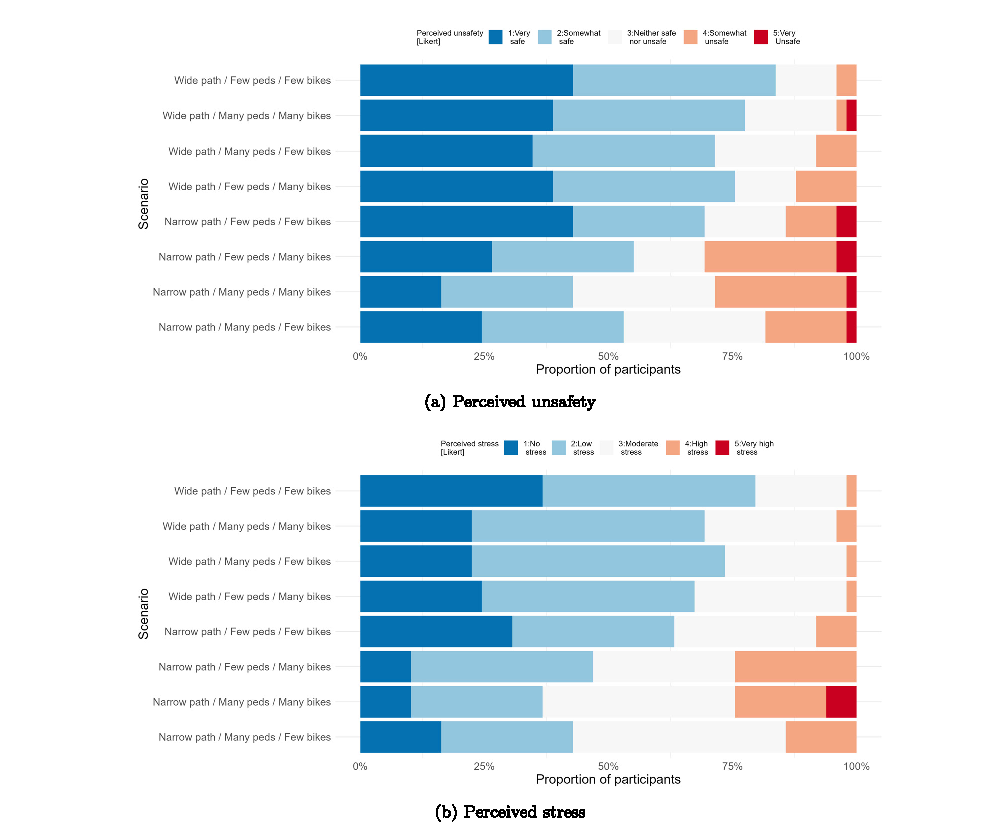
\includegraphics[width=0.86\linewidth]{figB9_unsafety_stress_shared.pdf}
  \caption{Perceived unsafety and stress in eight scenarios at the shared path
    environment.}
  \label{fig:b9}
\end{figure}

\begin{figure}[htbp]
  \centering
  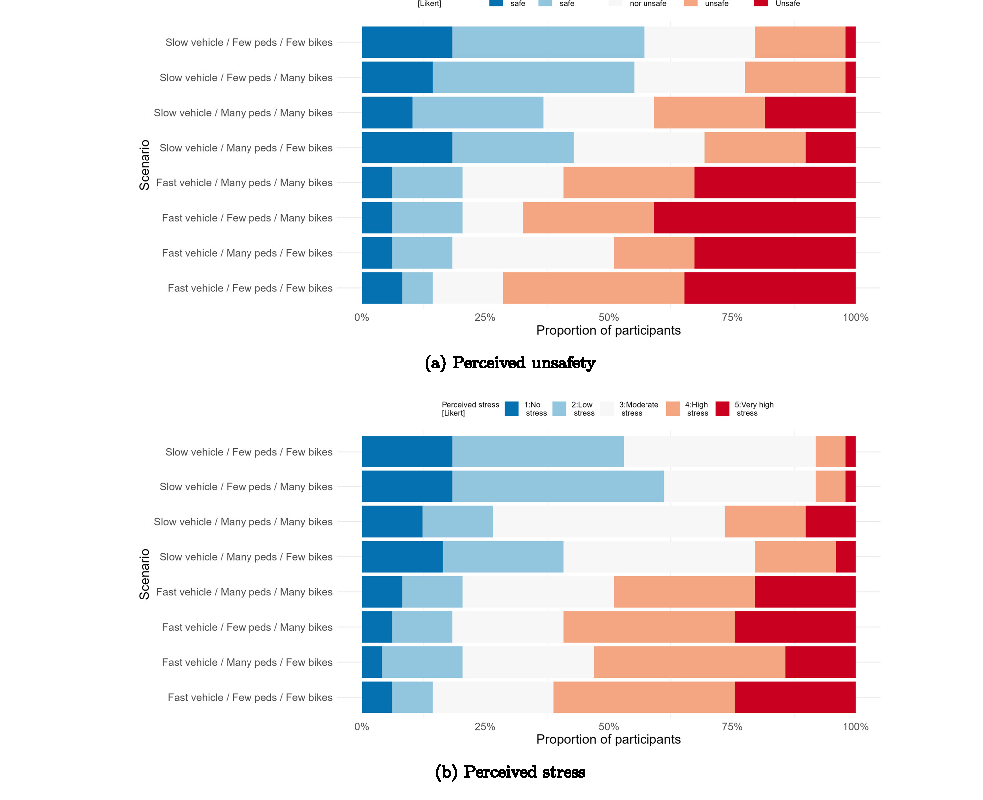
\includegraphics[width=0.86\linewidth]{figB10_unsafety_stress_unsig.pdf}
  \caption{Perceived unsafety and stress in eight scenarios at the unsignalized
    intersection environment.}
  \label{fig:b10}
\end{figure}

%---------------------------------------------------------------------
\section{Model estimation results with all variables}\label{app:allvariables}
%---------------------------------------------------------------------
\setcounter{table}{9}   % next table becomes C.10

See Tables~\ref{tab:c10}--\ref{tab:c14}.

\begin{table}[htbp]
  \centering
  \caption{Model estimation results for participant average speed at the shared
    path.}
  \label{tab:c10}
  \small
  \begin{threeparttable}
  \begin{tabular}{@{}l r r r l@{}}
    \toprule
    Variables & Coefficient & Std. error & t-value & p-value\\
    \midrule
    \multicolumn{5}{c}{Participant average speed [km/hour]}\\
    \addlinespace[2pt]
    Intercept                                        & 17.001 & 1.206 & 14.094 & \pvl\ ***\\
    Path width high                                  &  3.146 & 0.563 &  5.584 & \pvl\ ***\\
    Pedestrian flow high                             & -1.907 & 0.563 & -3.385 & 0.001 **\\
    Bicycle flow high                                & -1.050 & 0.563 & -1.864 & 0.063\\
    Road width high $\times$ Pedestrian flow high    &  0.314 & 0.651 &  0.482 & 0.630\\
    Path width high $\times$ Bicycle flow high       & -0.941 & 0.651 & -1.446 & 0.149\\
    Pedestrian flow high $\times$ Bicycle flow high  &  1.870 & 0.651 &  2.874 & 0.004 **\\
    \midrule
    \multicolumn{2}{@{}l}{Adjusted R-squared} & \multicolumn{3}{l}{0.485}\\
    \bottomrule
  \end{tabular}
  \begin{tablenotes}[flushleft]\footnotesize
    \item \sigstars
  \end{tablenotes}
  \end{threeparttable}
\end{table}

\begin{table}[htbp]
  \centering
  \caption{Model estimation results for perceived unsafety at the shared path.}
  \label{tab:c11}
  \small
  \begin{threeparttable}
  \begin{tabular}{@{}l r r r l@{}}
    \toprule
    Variables & Odds ratio & Std. error & t-value & p-value\\
    \midrule
    \multicolumn{2}{@{}l}{Intercepts (Thresholds)}
      & \multicolumn{3}{l}{Perceived unsafety [Likert]}\\
    \addlinespace[2pt]
    Perceived unsafety 1 vs 2 (or higher)             &   0.018 & 1.119 & -3.575 & \pvl\ ***\\
    Perceived unsafety 2 (or lower) vs 3 (or higher)  &   0.355 & 1.097 & -0.944 & 0.345\\
    Perceived unsafety 3 (or lower) vs 4 (or higher)  &   3.033 & 1.101 &  1.088 & 0.313\\
    Perceived unsafety 4 (or lower) vs 5              & 175.550 & 1.235 &  4.185 & \pvl\ ***\\
    \addlinespace[2pt]
    Participant average speed                         &   0.892 & 0.041 & -2.798 & 0.005 **\\
    Road Width high                                   &   0.655 & 0.436 & -0.972 & 0.331\\
    Bicycle flow high                                 &   4.982 & 0.434 &  3.697 & \pvl\ ***\\
    Pedestrian flow high                              &   3.947 & 0.422 &  3.254 & 0.001 **\\
    Fixation on pedestrians (\%)                      &   0.996 & 0.014 & -0.274 & 0.784\\
    Fixation on bicycles (\%)                         &   1.003 & 0.030 &  0.099 & 0.921\\
    Road Width high $\times$ Pedestrian flow high     &   0.437 & 0.474 & -1.749 & 0.080\\
    Road Width high $\times$ Bicycle flow high        &   0.327 & 0.476 & -2.374 & 0.018 *\\
    Bicycle flow high $\times$ Pedestrian flow high   &   0.530 & 0.457 & -1.335 & 0.182\\
    \midrule
    \multicolumn{2}{@{}l}{Akaike information criterion (AIC)}
      & \multicolumn{3}{l}{682.75}\\
    \bottomrule
  \end{tabular}
  \begin{tablenotes}[flushleft]\footnotesize
    \item \sigstars
  \end{tablenotes}
  \end{threeparttable}
\end{table}

\begin{table}[htbp]
  \centering
  \caption{Model estimation results for participant average speed at the
    unsignalized intersection.}
  \label{tab:c12}
  \small
  \begin{threeparttable}
  \begin{tabular}{@{}l r r r l@{}}
    \toprule
    Variables & Coefficient & Std. error & t-value & p-value\\
    \midrule
    \multicolumn{5}{c}{Participant average speed [km/hour]}\\
    \addlinespace[2pt]
    Intercept                                        & 16.023 & 1.621 &  9.883 & \pvl\ ***\\
    Vehicle speed high                               & -7.468 & 0.757 & -9.862 & \pvl\ ***\\
    Pedestrian flow high                             & -3.986 & 0.757 & -5.263 & \pvl\ ***\\
    Bicycle flow high                                & -0.754 & 0.757 & -0.996 & 0.320\\
    Vehicle speed high $\times$ Pedestrian flow high &  4.547 & 0.874 &  5.200 & \pvl\ ***\\
    Vehicle speed high $\times$ Bicycle flow high    &  1.579 & 0.874 &  1.806 & 0.072\\
    Pedestrian flow high $\times$ Bicycle flow high  &  1.000 & 0.874 &  1.144 & 0.254\\
    \midrule
    \multicolumn{2}{@{}l}{Adjusted R-squared} & \multicolumn{3}{l}{0.395}\\
    \bottomrule
  \end{tabular}
  \begin{tablenotes}[flushleft]\footnotesize
    \item \sigstars
  \end{tablenotes}
  \end{threeparttable}
\end{table}

\begin{table}[htbp]
  \centering
  \caption{Model estimation results for perceived unsafety at the unsignalized
    intersection.}
  \label{tab:c13}
  \small
  \begin{threeparttable}
  \begin{tabular}{@{}l r r r l@{}}
    \toprule
    Variables & Odds ratio & Std. error & t-value & p-value\\
    \midrule
    \multicolumn{2}{@{}l}{Intercepts (Thresholds)}
      & \multicolumn{3}{l}{Perceived unsafety [Likert]}\\
    \addlinespace[2pt]
    Perceived unsafety 1 vs 2 (or higher)             & 0.072 & 0.887 & -6.183 & \pvl\ ***\\
    Perceived unsafety 2 (or lower) vs 3 (or higher)  & 0.072 & 0.828 & -6.180 & \pvl\ ***\\
    Perceived unsafety 3 (or lower) vs 4 (or higher)  & 0.540 & 0.818 & -0.354 & 0.723\\
    Perceived unsafety 4 (or lower) vs 5              & 4.059 & 0.822 &  1.704 & 0.088\\
    \addlinespace[2pt]
    Participant average speed high                    & 0.795 & 0.033 & -7.028 & \pvl\ ***\\
    Vehicle speed high                                & 5.468 & 0.438 &  7.883 & \pvl\ ***\\
    Bicycle flow high                                 & 1.377 & 0.374 &  0.999 & 0.317\\
    Pedestrian flow high                              & 0.823 & 0.401 & -0.389 & 0.757\\
    Fixation on pedestrians (\%)                      & 1.020 & 0.014 &  1.369 & 0.171\\
    Fixation on bicycles (\%)                         & 0.868 & 0.044 & -1.495 & 0.135\\
    Fixation on vehicles (\%)                         & 1.055 & 0.020 &  2.716 & 0.007 **\\
    Vehicle speed high $\times$ Pedestrian flow high  & 0.600 & 0.458 & -2.111 & 0.035 *\\
    Vehicle speed high $\times$ Bicycle flow high     & 0.898 & 0.459 & -0.223 & 0.823\\
    Bicycle flow high $\times$ Pedestrian flow high   & 1.843 & 0.437 &  1.403 & 0.162\\
    \midrule
    \multicolumn{2}{@{}l}{Akaike information criterion (AIC)}
      & \multicolumn{3}{l}{834.31}\\
    \bottomrule
  \end{tabular}
  \begin{tablenotes}[flushleft]\footnotesize
    \item \sigstars
  \end{tablenotes}
  \end{threeparttable}
\end{table}

\begin{table}[htbp]
  \centering
  \caption{Model estimation results for fixation on vehicles at the unsignalized
    intersection.}
  \label{tab:c14}
  \small
  \begin{threeparttable}
  \begin{tabular}{@{}l r r r l@{}}
    \toprule
    Variables & Coefficient & Std. error & t-value & p-value\\
    \midrule
    \multicolumn{5}{c}{Fixation on vehicles [\%]}\\
    \addlinespace[2pt]
    Intercept                                        & 10.548 & 2.945 &  3.582 & \pvl\ ***\\
    Participant average speed high                   & -0.238 & 0.087 & -2.730 & 0.007 **\\
    Perceived unsafety high                          & -0.556 & 0.546 & -1.019 & 0.309\\
    Vehicle speed high                               &  4.257 & 1.382 &  3.080 & 0.002 **\\
    Pedestrian flow high                             & -1.489 & 1.282 & -1.162 & 0.246\\
    Bicycle flow high                                & -0.363 & 1.215 & -0.299 & 0.765\\
    Vehicle speed high $\times$ Pedestrian flow high & -0.701 & 1.457 & -0.481 & 0.631\\
    Vehicle speed high $\times$ Bicycle flow high    & -0.175 & 1.424 & -0.123 & 0.902\\
    Pedestrian flow high $\times$ Bicycle flow high  & -0.465 & 1.419 & -0.328 & 0.743\\
    \midrule
    \multicolumn{2}{@{}l}{Adjusted R-squared} & \multicolumn{3}{l}{0.579}\\
    \bottomrule
  \end{tabular}
  \begin{tablenotes}[flushleft]\footnotesize
    \item \sigstars
  \end{tablenotes}
  \end{threeparttable}
\end{table}


%=====================================================================
% References
%=====================================================================
%=====================================================================
%  Reference list, formatted to match the published article (APA-style,
%  the house style of Transportation Research Part F).
%
%  natbib label syntax:  \bibitem[Short(Year)Long]{key}
%    \citep{key}  -> "(Short, Year)"      e.g. "(Buehler & Pucher, 2021)"
%    \citet{key}  -> "Short (Year)"
%    \citet*{key} -> "Long (Year)"        e.g. "Buehler and Pucher (2021)"
%  The short form carries "&" (used inside parentheses) and the long form
%  carries "and" (used in running text), exactly as in the article. Use
%  \citet* for narrative citations of two-author works.
%
%  refs.bib carries the same entries in BibTeX form.
%=====================================================================

\begin{thebibliography}{99}
\setlength{\itemsep}{1pt plus 0.2pt}

\bibitem[Andersen et al.(2012)]{andersen2012collection}
Andersen, T., Breda, F., Weinreich, M., Jensen, N., Riisgaard-Dam, M., \&
Nielsen, M. K. (2012). \emph{Collection of cycle concepts 2012}. Technical
Report. Cycling Embassy of Denmark.
\url{https://bicycleinfrastructuremanuals.com/manuals1/Collection-of-Cycle-Concepts-2012_Denmark.pdf}.

\bibitem[Ballo et al.(2023)]{ballo2023ebike}
Ballo, L., de Freitas, L. M., Meister, A., \& Axhausen, K. W. (2023). The E-Bike
city as a radical shift toward zero-emission transport: Sustainable? Equitable?
Desirable? \emph{Journal of Transport Geography, 111}, Article 103663.
\url{https://doi.org/10.1016/j.jtrangeo.2023.103663}.
\url{https://www.sciencedirect.com/science/article/pii/S0966692323001357}.

\bibitem[Batista et al.(2023)]{batista2023exploring}
Batista, M., Berghoefer, F. L., \& Friedrich, B. (2023). Exploring pedestrian
and cyclist preferences for shared space design: A video-based online survey.
\emph{Transportation Research Interdisciplinary Perspectives, 22}, Article
100976. \url{https://doi.org/10.1016/j.trip.2023.100976}.

\bibitem[Beitel et al.(2018)]{beitel2018assessing}
Beitel, D., Stipancic, J., Manaugh, K., \& Miranda-Moreno, L. (2018). Assessing
safety of shared space using cyclist-pedestrian interactions and automated video
conflict analysis. \emph{Transportation Research. Part D, Transport and
Environment, 65}, 710--724. \url{https://doi.org/10.1016/j.trd.2018.10.001}.
\url{https://linkinghub.elsevier.com/retrieve/pii/S1361920917301694}.

\bibitem[Berghoefer \& Vollrath(2023)Berghoefer and Vollrath]{berghoefer2023prefer}
Berghoefer, F. L., \& Vollrath, M. (2023). Prefer what you like? Evaluation and
preference of cycling infrastructures in a bicycle simulator. \emph{Journal of
Safety Research}. \url{https://doi.org/10.1016/j.jsr.2023.09.013}.
\url{https://www.sciencedirect.com/science/article/pii/S0022437523001421}.

\bibitem[Beura et al.(2021)]{beura2021unsignalized}
Beura, S. K., Srivastava, A., \& Bhuyan, P. K. (2021). Unsignalized intersection
level of service: A bicyclist's perspective. \emph{International Journal of
Intelligent Transport Systems Research, 19}, 405--416.
\url{https://doi.org/10.1007/s13177-020-00244-z}.
\url{https://link.springer.com/10.1007/s13177-020-00244-z}.

\bibitem[Bogacz et al.(2020)]{bogacz2020comparison}
Bogacz, M., Hess, S., Calastri, C., Choudhury, C. F., Erath, A., van Eggermond,
M. A. B., Mushtaq, F., Nazemi, M., \& Awais, M. (2020). Comparison of cycling
behavior between keyboard-controlled and instrumented bicycle experiments in
virtual reality. \emph{Transportation Research Record, 2674}, 244--257.
\url{https://doi.org/10.1177/0361198120921850}. Publisher: SAGE Publications
Inc.

\bibitem[Boufous et al.(2018)]{boufous2018impact}
Boufous, S., Hatfield, J., \& Grzebieta, R. (2018). The impact of environmental
factors on cycling speed on shared paths. \emph{Accident Analysis and
Prevention, 110}, 171--176. \url{https://doi.org/10.1016/j.aap.2017.09.017}.
\url{https://www.sciencedirect.com/science/article/pii/S000145751730338X}.

\bibitem[Buehler \& Pucher(2008)Buehler and Pucher]{buehler2008making}
Buehler, R., \& Pucher, J. (2008). Making cycling irresistible: Lessons from the
Netherlands, Denmark and Germany. \emph{Transport Reviews, 28}, 495--528.
\url{https://doi.org/10.1080/01441640701806612}.

\bibitem[Buehler \& Pucher(2021)Buehler and Pucher]{buehler2021covid}
Buehler, R., \& Pucher, J. (2021). COVID-19 impacts on cycling, 2019--2020.
\emph{Transport Reviews, 41}, 393--400.
\url{https://doi.org/10.1080/01441647.2021.1914900}.

\bibitem[Che et al.(2021)]{che2021interaction}
Che, M., Wong, Y. D., Lum, K. M., \& Wang, X. (2021). Interaction behaviour of
active mobility users in shared space. \emph{Transportation Research. Part A,
Policy and Practice, 153}, 52--65.
\url{https://doi.org/10.1016/j.tra.2021.08.017}.
\url{https://linkinghub.elsevier.com/retrieve/pii/S0965856421002238}. Publisher:
Elsevier BV.

\bibitem[Chou et al.(2024)]{chou2024comparative}
Chou, K. Y., Paulsen, M., Jensen, A. F., Rasmussen, T. K., \& Nielsen, O. A.
(2024). Comparative modeling of risk factors for near-crashes from crowdsourced
bicycle airbag helmet data and crashes from conventional police data.
\emph{Journal of Safety Research, 91}, 465--480.
\url{https://doi.org/10.1016/j.jsr.2024.10.003}.
\url{https://linkinghub.elsevier.com/retrieve/pii/S0022437524001439}.

\bibitem[Cobb et al.(2021)]{cobb2021bicyclists}
Cobb, D. P., Jashami, H., \& Hurwitz, D. S. (2021). Bicyclists' behavioral and
physiological responses to varying roadway conditions and bicycle
infrastructure. \emph{Transportation Research. Part F, Traffic Psychology and
Behaviour, 80}, 172--188. \url{https://doi.org/10.1016/j.trf.2021.04.004}.
\url{https://www.sciencedirect.com/science/article/pii/S1369847821000851}.

\bibitem[Commission(2024)]{ec2024speed}
Commission, E. (2024). \emph{Current speed limit policies -- European
commission}.
\url{https://road-safety.transport.ec.europa.eu/eu-road-safety-policy/priorities/safe-road-use/safe-speed/archive/current-speed-limit-policies_en}.

\bibitem[Cyclenation(2014)]{cyclenation2014}
Cyclenation (2014). \emph{Making space for cycling -- a guide for new
developments and street renewals}. Technical Report.
\url{https://www.makingspaceforcycling.org/}.

\bibitem[Damien Masson(2024)]{masson2024latin}
Damien Masson (2024). \emph{Balanced Latin square online generator}.
\url{https://damienmasson.com/tools/latin_square/}.

\bibitem[Essa et al.(2018)]{essa2018road}
Essa, M., Hussein, M., \& Sayed, T. (2018). Road users' behavior and safety
analysis of pedestrian--bike shared space: Case study of Robson street in
Vancouver. \emph{Canadian Journal of Civil Engineering, 45}, 1053--1064.
\url{https://doi.org/10.1139/cjce-2017-0683}.
\url{http://www.nrcresearchpress.com/doi/10.1139/cjce-2017-0683}.

\bibitem[FGSV(2010)]{fgsv2010}
FGSV (2010). \emph{Empfehlungen für Radverkehrsanlagen}. Technical Report.
Forschungsgesellschaft für Straßen- und Verkehrswesen.
\url{https://www.fgsv-verlag.de/era}.

\bibitem[Friel et al.(2023)]{friel2023cyclists}
Friel, D., Wachholz, S., Werner, T., Zimmermann, L., Schwedes, O., \& Stark, R.
(2023). Cyclists' perceived safety on intersections and roundabouts -- a
qualitative bicycle simulator study. \emph{Journal of Safety Research, 87},
143--156. \url{https://doi.org/10.1016/j.jsr.2023.09.012}.
\url{https://www.sciencedirect.com/science/article/pii/S002243752300141X}.

\bibitem[Gkekas et al.(2020)]{gkekas2020perceived}
Gkekas, F., Bigazzi, A., \& Gill, G. (2020). Perceived safety and experienced
incidents between pedestrians and cyclists in a high-volume non-motorized shared
space. \emph{Transportation Research Interdisciplinary Perspectives, 4}, Article
100094. \url{https://doi.org/10.1016/j.trip.2020.100094}.
\url{https://www.sciencedirect.com/science/article/pii/S2590198220300051}.

\bibitem[Guo et al.(2023)]{guo2023psycho}
Guo, X., Tavakoli, A., Angulo, A., Robartes, E., Chen, T. D., \& Heydarian, A.
(2023). Psycho-physiological measures on a bicycle simulator in immersive
virtual environments: How protected/curbside bike lanes may improve perceived
safety. \emph{Transportation Research. Part F, Traffic Psychology and Behaviour,
92}, 317--336. \url{https://doi.org/10.1016/j.trf.2022.11.015}.
\url{https://www.sciencedirect.com/science/article/pii/S1369847822002832}.

\bibitem[Hamilton-Baillie(2008)]{hamiltonbaillie2008shared}
Hamilton-Baillie, B. (2008). Shared space: Reconciling people, places and
traffic. \emph{Built Environment, 34}, 161--181.
\url{https://doi.org/10.2148/benv.34.2.161}.

\bibitem[Huang et al.(2021)]{huang2021investigating}
Huang, C., Wang, L., Yu, H., Li, H., Zhang, J., Song, W., Lo, S., \& Rafaqat, W.
(2021). Investigating the influence of a cyclist on crowd behaviors on a shared
road. \emph{Journal of Statistical Mechanics: Theory and Experiment, 2021},
Article 083402. \url{https://doi.org/10.1088/1742-5468/ac0edd}.
\url{https://dx.doi.org/10.1088/1742-5468/ac0edd}. Publisher: IOP Publishing and
SISSA.

\bibitem[Hummer et al.(2005)]{hummer2005user}
Hummer, J. E., Rouphail, N., Hughes, R. G., Fain, S. J., Toole, J. L., Patten,
R. S., Schneider, R. J., Monahan, J. F., \& Do, A. (2005). User perceptions of
the quality of service on shared paths. \emph{Transportation Research Record,
1939}, 28--36. \url{https://doi.org/10.1177/0361198105193900104}. Publisher:
SAGE Publications Inc.

\bibitem[Jensen(2012)]{jensen2012pedestrian}
Jensen, S. U. (2012). \emph{Pedestrian and bicycle level of service at
intersections, roundabouts and other crossings}. Technical Report. Trafitec.
\url{https://trafitec.dk/wp-content/uploads/2023/07/158-Pedestrian-and-Bicycle-Level-of-Service-at-Intersections-Roundabouts-and-other-Crossings.pdf}.

\bibitem[Kazemzadeh et al.(2024)]{kazemzadeh2024forwhom}
Kazemzadeh, K., Afghari, A. P., \& Cherry, C. R. (2024). For whom is sharing
really scaring? Capturing unobserved heterogeneity in perceived comfort when
cycling in shared spaces. \emph{Transportation Research. Part F, Traffic
Psychology and Behaviour, 103}, 306--318.
\url{https://doi.org/10.1016/j.trf.2024.04.017}.

\bibitem[Keler et al.(2018)]{keler2018bicycle}
Keler, A., Kaths, J., Chucholowski, F., Chucholowski, M., Grigoropoulos, G.,
Spangler, M., Kaths, H., \& Busch, F. (2018). A bicycle simulator for
experiencing microscopic traffic flow simulation in urban environments. In
\emph{2018 21st international conference on intelligent transportation systems
(ITSC)} (pp. 3020--3023). Maui, HI: IEEE.
\url{https://ieeexplore.ieee.org/document/8569576/}.

\bibitem[Kwigizile et al.(2017)]{kwigizile2017real}
Kwigizile, V., Oh, J. S., Ikonomov, P., Hasan, R., Villalobos, C. G., Kurdi,
A. H., \& Shaw, A. (2017). \emph{Real time bicycle simulation study of
bicyclists' behaviors and their implication on safety}. Technical Report TRCLC
2015-03. Western Michigan University.
\url{https://rosap.ntl.bts.gov/view/dot/34885}.

\bibitem[Liu et al.(2012)]{liu2012response}
Liu, W. C., Jeng, M. C., Hwang, J. R., Doong, J. L., Lin, C. Y., \& Lai, C. H.
(2012). The response patterns of young bicyclists to a right-turning motorcycle:
A simulator study. \emph{Perceptual and Motor Skills, 115}, 385--402.
\url{https://doi.org/10.2466/22.25.27.PMS.115.5.385-402}. Publisher: SAGE
Publications Inc.

\bibitem[Mesimäki \& Luoma(2021)Mesimäki and Luoma]{mesimaki2021near}
Mesimäki, J., \& Luoma, J. (2021). Near accidents and collisions between
pedestrians and cyclists. \emph{European Transport Research Review, 13}, 38.
\url{https://doi.org/10.1186/s12544-021-00497-z}.
\url{https://etrr.springeropen.com/articles/10.1186/s12544-021-00497-z}.

\bibitem[Meuleners \& Fraser(2015)Meuleners and Fraser]{meuleners2015validation}
Meuleners, L., \& Fraser, M. (2015). A validation study of driving errors using
a driving simulator. \emph{Transportation Research. Part F, Traffic Psychology
and Behaviour, 29}, 14--21. \url{https://doi.org/10.1016/j.trf.2014.11.009}.
\url{https://www.sciencedirect.com/science/article/pii/S1369847814001764}.

\bibitem[Meuleners et al.(2023)]{meuleners2023improving}
Meuleners, L., Fraser, M., \& Roberts, P. (2023). Improving cycling safety
through infrastructure design: A bicycle simulator study. \emph{Transportation
Research Interdisciplinary Perspectives, 18}, Article 100768.
\url{https://doi.org/10.1016/j.trip.2023.100768}.
\url{https://www.sciencedirect.com/science/article/pii/S2590198223000155}.

\bibitem[Mohammadi et al.(2023)]{mohammadi2023how}
Mohammadi, A., Bianchi Piccinini, G., \& Dozza, M. (2023). How do cyclists
interact with motorized vehicles at unsignalized intersections? Modeling
cyclists' yielding behavior using naturalistic data. \emph{Accident Analysis and
Prevention, 190}, Article 107156.
\url{https://doi.org/10.1016/j.aap.2023.107156}.
\url{https://www.sciencedirect.com/science/article/pii/S0001457523002038}.

\bibitem[Mohammadi et al.(2024)]{mohammadi2024understanding}
Mohammadi, A., Bianchi Piccinini, G., \& Dozza, M. (2024). Understanding the
interaction between cyclists and motorized vehicles at unsignalized
intersections: Results from a cycling simulator study. \emph{Journal of Safety
Research, 90}, 306--318. \url{https://doi.org/10.1016/j.jsr.2024.05.007}.
\url{https://www.sciencedirect.com/science/article/pii/S0022437524000604}.

\bibitem[Nazemi et al.(2021)]{nazemi2021studying}
Nazemi, M., van Eggermond, M. A. B., Erath, A., Schaffner, D., Joos, M., \&
Axhausen, K. W. (2021). Studying bicyclists' perceived level of safety using a
bicycle simulator combined with immersive virtual reality. \emph{Accident
Analysis and Prevention, 151}, Article 105943.
\url{https://doi.org/10.1016/j.aap.2020.105943}.
\url{https://www.sciencedirect.com/science/article/pii/S0001457520317632}.

\bibitem[Negi \& Mitra(2020)Negi and Mitra]{negi2020fixation}
Negi, S., \& Mitra, R. (2020). Fixation duration and the learning process: An
eye tracking study with subtitled videos. \emph{Journal of Eye Movement
Research, 13}. \url{https://doi.org/10.16910/jemr.13.6.1}.
\url{https://www.ncbi.nlm.nih.gov/pmc/articles/PMC8012014/}.

\bibitem[Ng et al.(2017)]{ng2017cyclist}
Ng, A., Debnath, A. K., \& Heesch, K. C. (2017). Cyclist' safety perceptions of
cycling infrastructure at un-signalised intersections: Cross-sectional survey of
Queensland cyclists. \emph{Journal of Transport \& Health, 6}, 13--22.
\url{https://doi.org/10.1016/j.jth.2017.03.001}.
\url{https://www.sciencedirect.com/science/article/pii/S2214140516303188}.

\bibitem[Nikiforiadis \& Basbas(2019)Nikiforiadis and Basbas]{nikiforiadis2019can}
Nikiforiadis, A., \& Basbas, S. (2019). Can pedestrians and cyclists share the
same space? The case of a city with low cycling levels and experience.
\emph{Sustainable Cities and Society, 46}, Article 101453.
\url{https://doi.org/10.1016/j.scs.2019.101453}.

\bibitem[O'Hern et al.(2017)]{ohern2017validation}
O'Hern, S., Oxley, J., \& Stevenson, M. (2017). Validation of a bicycle
simulator for road safety research. \emph{Accident Analysis and Prevention,
100}, 53--58. \url{https://doi.org/10.1016/j.aap.2017.01.002}.
\url{https://www.sciencedirect.com/science/article/pii/S0001457517300027}.

\bibitem[Pashkevich et al.(2022)]{pashkevich2022visual}
Pashkevich, A., Burghardt, T. E., Puławska-Obiedowska, S., \& Šucha, M. (2022).
Visual attention and speeds of pedestrians, cyclists, and electric scooter
riders when using shared road -- a field eye tracker experiment. \emph{Case
Studies on Transport Policy, 10}, 549--558.
\url{https://doi.org/10.1016/j.cstp.2022.01.015}.

\bibitem[Poulos et al.(2017)]{poulos2017near}
Poulos, R. G., Hatfield, J., Rissel, C., Flack, L. K., Shaw, L., Grzebieta, R.,
\& McIntosh, A. S. (2017). Near miss experiences of transport and recreational
cyclists in New South Wales, Australia. Findings from a prospective cohort
study. \emph{Accident Analysis and Prevention, 101}, 143--153.
\url{https://doi.org/10.1016/j.aap.2017.01.020}.
\url{https://www.sciencedirect.com/science/article/pii/S0001457517300477}.

\bibitem[Pupil Core(2024)]{pupilcore2024}
Pupil Core (2024). \emph{Open source eye tracking platform}.
\url{https://pupil-labs.com/products/core}.

\bibitem[RoadRunner(2024)]{roadrunner2024}
RoadRunner (2024). \emph{RoadRunner}.
\url{https://de.mathworks.com/products/roadrunner.html}.

\bibitem[Scott-Deeter et al.(2023)]{scottdeeter2023assessing}
Scott-Deeter, L., Hurwitz, D., Russo, B., Smaglik, E., \& Kothuri, S. (2023).
Assessing the impact of three intersection treatments on bicyclist safety using
a bicycling simulator. \emph{Accident Analysis and Prevention, 179}, Article
106877. \url{https://doi.org/10.1016/j.aap.2022.106877}.
\url{https://www.sciencedirect.com/science/article/pii/S0001457522003128}.

\bibitem[Skoczyński(2021)]{skoczynski2021analysis}
Skoczyński, P. (2021). Analysis of solutions improving safety of cyclists in the
road traffic. \emph{Applied Sciences, 11}, 3771.
\url{https://doi.org/10.3390/app11093771}.
\url{https://www.mdpi.com/2076-3417/11/9/3771}.

\bibitem[Stülpnagel(2020)]{stulpnagel2020gaze}
Stülpnagel, R. (2020). Gaze behavior during urban cycling: Effects of subjective
risk perception and vista space properties. \emph{Transportation Research. Part
F, Traffic Psychology and Behaviour, 75}, 222--238.
\url{https://doi.org/10.1016/j.trf.2020.10.003}.

\bibitem[von Stülpnagel \& Rintelen(2024)von Stülpnagel and Rintelen]{vonstulpnagel2024matter}
von Stülpnagel, R., \& Rintelen, H. (2024). A matter of space and perspective --
cyclists', car drivers', and pedestrians' assumptions about subjective safety in
shared traffic situations. \emph{Transportation Research. Part A, Policy and
Practice, 179}, Article 103941.
\url{https://doi.org/10.1016/j.tra.2023.103941}.
\url{https://www.sciencedirect.com/science/article/pii/S0965856423003610}.

\bibitem[Suzuki et al.(2018)]{suzuki2018fundamental}
Suzuki, M., Sato, K., Hosoya, K., Miyanoue, K., \& Yai, T. (2018). \emph{A
fundamental study of validation of cycling simulator and designing safety
education programs}. \url{https://trid.trb.org/view/1495332}. Number: 18-02484.

\bibitem[Takanashi \& Murao(2018)Takanashi and Murao]{takanashi2018analysis}
Takanashi, H., \& Murao, I. (2018). Analysis of near-miss incidents between car
and bicycle at non-intersection. In \emph{Proceedings of international conference
on technology and social science 2018 (ICTSS 2018)}.
\url{http://conf.e-jikei.org/ICTSS2018/proceedings/materials/proc_files/IPS09\%5BHashimoto\%5D/ICTSS2018-IPS09-05/IPS09_05_takanashi.pdf}.

\bibitem[Velichkovsky et al.(2002)]{velichkovsky2002towards}
Velichkovsky, B. M., Rothert, A., Kopf, M., Dornhöfer, S. M., \& Joos, M.
(2002). Towards an express-diagnostics for level of processing and hazard
perception. \emph{Transportation Research. Part F, Traffic Psychology and
Behaviour, 5}, 145--156.
\url{https://doi.org/10.1016/S1369-8478(02)00013-X}.
\url{https://www.sciencedirect.com/science/article/pii/S136984780200013X}.

\bibitem[Wongwaiwit et al.(2011)]{wongwaiwit2011analysis}
Wongwaiwit, P., Michitsuji, Y., \& Raksincharoensak, Pongsathorn (2011).
Analysis on pedestrian and bicycle behavior in unsignalized intersection based
on near-miss incident database. In \emph{The proceedings of the transportation
and logistics conference 2011.20} (pp. 19--22).
\url{https://www.jstage.jst.go.jp/article/jsmetld/2011.20/0/2011.20_19/_article}.

\bibitem[Xu et al.(2023)]{xu2023assessing}
Xu, Z., Zheng, N., Logan, D. B., \& Vu, H. L. (2023). Assessing bicycle-vehicle
conflicts at urban intersections utilizing a VR integrated simulation approach.
\emph{Accident Analysis and Prevention, 191}, Article 107194.
\url{https://doi.org/10.1016/j.aap.2023.107194}.
\url{https://www.sciencedirect.com/science/article/pii/S0001457523002415}.

\bibitem[Zeuwts et al.(2023)]{zeuwts2023using}
Zeuwts, L. H. R. H., Vanhuele, R., Vansteenkiste, P., Deconinck, F. J. A., \&
Lenoir, M. (2023). Using an immersive virtual reality bicycle simulator to
evaluate hazard detection and anticipation of overt and covert traffic
situations in young bicyclists. \emph{Virtual Reality, 27}, 1507--1527.
\url{https://doi.org/10.1007/s10055-023-00746-7}.

\bibitem[Zhang et al.(2023)]{zhang2023space}
Zhang, C., Du, B., Zheng, Z., \& Shen, J. (2023). Space sharing between
pedestrians and micro-mobility vehicles: A systematic review.
\emph{Transportation Research. Part D, Transport and Environment, 116}, Article
103629. \url{https://doi.org/10.1016/j.trd.2023.103629}.
\url{https://www.sciencedirect.com/science/article/pii/S1361920923000263}.

\bibitem[Zhang et al.(2017)]{zhang2017study}
Zhang, R., Wu, J., Huang, L., \& You, F. (2017). Study of bicycle movements in
conflicts at mixed traffic unsignalized intersections. \emph{IEEE Access, 5},
10108--10117. \url{https://doi.org/10.1109/ACCESS.2017.2703816}.
\url{https://ieeexplore.ieee.org/document/7927409/}. Publisher: IEEE.

\end{thebibliography}


% BibTeX alternative -- delete %=====================================================================
%  Reference list, formatted to match the published article (APA-style,
%  the house style of Transportation Research Part F).
%
%  natbib label syntax:  \bibitem[Short(Year)Long]{key}
%    \citep{key}  -> "(Short, Year)"      e.g. "(Buehler & Pucher, 2021)"
%    \citet{key}  -> "Short (Year)"
%    \citet*{key} -> "Long (Year)"        e.g. "Buehler and Pucher (2021)"
%  The short form carries "&" (used inside parentheses) and the long form
%  carries "and" (used in running text), exactly as in the article. Use
%  \citet* for narrative citations of two-author works.
%
%  refs.bib carries the same entries in BibTeX form.
%=====================================================================

\begin{thebibliography}{99}
\setlength{\itemsep}{1pt plus 0.2pt}

\bibitem[Andersen et al.(2012)]{andersen2012collection}
Andersen, T., Breda, F., Weinreich, M., Jensen, N., Riisgaard-Dam, M., \&
Nielsen, M. K. (2012). \emph{Collection of cycle concepts 2012}. Technical
Report. Cycling Embassy of Denmark.
\url{https://bicycleinfrastructuremanuals.com/manuals1/Collection-of-Cycle-Concepts-2012_Denmark.pdf}.

\bibitem[Ballo et al.(2023)]{ballo2023ebike}
Ballo, L., de Freitas, L. M., Meister, A., \& Axhausen, K. W. (2023). The E-Bike
city as a radical shift toward zero-emission transport: Sustainable? Equitable?
Desirable? \emph{Journal of Transport Geography, 111}, Article 103663.
\url{https://doi.org/10.1016/j.jtrangeo.2023.103663}.
\url{https://www.sciencedirect.com/science/article/pii/S0966692323001357}.

\bibitem[Batista et al.(2023)]{batista2023exploring}
Batista, M., Berghoefer, F. L., \& Friedrich, B. (2023). Exploring pedestrian
and cyclist preferences for shared space design: A video-based online survey.
\emph{Transportation Research Interdisciplinary Perspectives, 22}, Article
100976. \url{https://doi.org/10.1016/j.trip.2023.100976}.

\bibitem[Beitel et al.(2018)]{beitel2018assessing}
Beitel, D., Stipancic, J., Manaugh, K., \& Miranda-Moreno, L. (2018). Assessing
safety of shared space using cyclist-pedestrian interactions and automated video
conflict analysis. \emph{Transportation Research. Part D, Transport and
Environment, 65}, 710--724. \url{https://doi.org/10.1016/j.trd.2018.10.001}.
\url{https://linkinghub.elsevier.com/retrieve/pii/S1361920917301694}.

\bibitem[Berghoefer \& Vollrath(2023)Berghoefer and Vollrath]{berghoefer2023prefer}
Berghoefer, F. L., \& Vollrath, M. (2023). Prefer what you like? Evaluation and
preference of cycling infrastructures in a bicycle simulator. \emph{Journal of
Safety Research}. \url{https://doi.org/10.1016/j.jsr.2023.09.013}.
\url{https://www.sciencedirect.com/science/article/pii/S0022437523001421}.

\bibitem[Beura et al.(2021)]{beura2021unsignalized}
Beura, S. K., Srivastava, A., \& Bhuyan, P. K. (2021). Unsignalized intersection
level of service: A bicyclist's perspective. \emph{International Journal of
Intelligent Transport Systems Research, 19}, 405--416.
\url{https://doi.org/10.1007/s13177-020-00244-z}.
\url{https://link.springer.com/10.1007/s13177-020-00244-z}.

\bibitem[Bogacz et al.(2020)]{bogacz2020comparison}
Bogacz, M., Hess, S., Calastri, C., Choudhury, C. F., Erath, A., van Eggermond,
M. A. B., Mushtaq, F., Nazemi, M., \& Awais, M. (2020). Comparison of cycling
behavior between keyboard-controlled and instrumented bicycle experiments in
virtual reality. \emph{Transportation Research Record, 2674}, 244--257.
\url{https://doi.org/10.1177/0361198120921850}. Publisher: SAGE Publications
Inc.

\bibitem[Boufous et al.(2018)]{boufous2018impact}
Boufous, S., Hatfield, J., \& Grzebieta, R. (2018). The impact of environmental
factors on cycling speed on shared paths. \emph{Accident Analysis and
Prevention, 110}, 171--176. \url{https://doi.org/10.1016/j.aap.2017.09.017}.
\url{https://www.sciencedirect.com/science/article/pii/S000145751730338X}.

\bibitem[Buehler \& Pucher(2008)Buehler and Pucher]{buehler2008making}
Buehler, R., \& Pucher, J. (2008). Making cycling irresistible: Lessons from the
Netherlands, Denmark and Germany. \emph{Transport Reviews, 28}, 495--528.
\url{https://doi.org/10.1080/01441640701806612}.

\bibitem[Buehler \& Pucher(2021)Buehler and Pucher]{buehler2021covid}
Buehler, R., \& Pucher, J. (2021). COVID-19 impacts on cycling, 2019--2020.
\emph{Transport Reviews, 41}, 393--400.
\url{https://doi.org/10.1080/01441647.2021.1914900}.

\bibitem[Che et al.(2021)]{che2021interaction}
Che, M., Wong, Y. D., Lum, K. M., \& Wang, X. (2021). Interaction behaviour of
active mobility users in shared space. \emph{Transportation Research. Part A,
Policy and Practice, 153}, 52--65.
\url{https://doi.org/10.1016/j.tra.2021.08.017}.
\url{https://linkinghub.elsevier.com/retrieve/pii/S0965856421002238}. Publisher:
Elsevier BV.

\bibitem[Chou et al.(2024)]{chou2024comparative}
Chou, K. Y., Paulsen, M., Jensen, A. F., Rasmussen, T. K., \& Nielsen, O. A.
(2024). Comparative modeling of risk factors for near-crashes from crowdsourced
bicycle airbag helmet data and crashes from conventional police data.
\emph{Journal of Safety Research, 91}, 465--480.
\url{https://doi.org/10.1016/j.jsr.2024.10.003}.
\url{https://linkinghub.elsevier.com/retrieve/pii/S0022437524001439}.

\bibitem[Cobb et al.(2021)]{cobb2021bicyclists}
Cobb, D. P., Jashami, H., \& Hurwitz, D. S. (2021). Bicyclists' behavioral and
physiological responses to varying roadway conditions and bicycle
infrastructure. \emph{Transportation Research. Part F, Traffic Psychology and
Behaviour, 80}, 172--188. \url{https://doi.org/10.1016/j.trf.2021.04.004}.
\url{https://www.sciencedirect.com/science/article/pii/S1369847821000851}.

\bibitem[Commission(2024)]{ec2024speed}
Commission, E. (2024). \emph{Current speed limit policies -- European
commission}.
\url{https://road-safety.transport.ec.europa.eu/eu-road-safety-policy/priorities/safe-road-use/safe-speed/archive/current-speed-limit-policies_en}.

\bibitem[Cyclenation(2014)]{cyclenation2014}
Cyclenation (2014). \emph{Making space for cycling -- a guide for new
developments and street renewals}. Technical Report.
\url{https://www.makingspaceforcycling.org/}.

\bibitem[Damien Masson(2024)]{masson2024latin}
Damien Masson (2024). \emph{Balanced Latin square online generator}.
\url{https://damienmasson.com/tools/latin_square/}.

\bibitem[Essa et al.(2018)]{essa2018road}
Essa, M., Hussein, M., \& Sayed, T. (2018). Road users' behavior and safety
analysis of pedestrian--bike shared space: Case study of Robson street in
Vancouver. \emph{Canadian Journal of Civil Engineering, 45}, 1053--1064.
\url{https://doi.org/10.1139/cjce-2017-0683}.
\url{http://www.nrcresearchpress.com/doi/10.1139/cjce-2017-0683}.

\bibitem[FGSV(2010)]{fgsv2010}
FGSV (2010). \emph{Empfehlungen für Radverkehrsanlagen}. Technical Report.
Forschungsgesellschaft für Straßen- und Verkehrswesen.
\url{https://www.fgsv-verlag.de/era}.

\bibitem[Friel et al.(2023)]{friel2023cyclists}
Friel, D., Wachholz, S., Werner, T., Zimmermann, L., Schwedes, O., \& Stark, R.
(2023). Cyclists' perceived safety on intersections and roundabouts -- a
qualitative bicycle simulator study. \emph{Journal of Safety Research, 87},
143--156. \url{https://doi.org/10.1016/j.jsr.2023.09.012}.
\url{https://www.sciencedirect.com/science/article/pii/S002243752300141X}.

\bibitem[Gkekas et al.(2020)]{gkekas2020perceived}
Gkekas, F., Bigazzi, A., \& Gill, G. (2020). Perceived safety and experienced
incidents between pedestrians and cyclists in a high-volume non-motorized shared
space. \emph{Transportation Research Interdisciplinary Perspectives, 4}, Article
100094. \url{https://doi.org/10.1016/j.trip.2020.100094}.
\url{https://www.sciencedirect.com/science/article/pii/S2590198220300051}.

\bibitem[Guo et al.(2023)]{guo2023psycho}
Guo, X., Tavakoli, A., Angulo, A., Robartes, E., Chen, T. D., \& Heydarian, A.
(2023). Psycho-physiological measures on a bicycle simulator in immersive
virtual environments: How protected/curbside bike lanes may improve perceived
safety. \emph{Transportation Research. Part F, Traffic Psychology and Behaviour,
92}, 317--336. \url{https://doi.org/10.1016/j.trf.2022.11.015}.
\url{https://www.sciencedirect.com/science/article/pii/S1369847822002832}.

\bibitem[Hamilton-Baillie(2008)]{hamiltonbaillie2008shared}
Hamilton-Baillie, B. (2008). Shared space: Reconciling people, places and
traffic. \emph{Built Environment, 34}, 161--181.
\url{https://doi.org/10.2148/benv.34.2.161}.

\bibitem[Huang et al.(2021)]{huang2021investigating}
Huang, C., Wang, L., Yu, H., Li, H., Zhang, J., Song, W., Lo, S., \& Rafaqat, W.
(2021). Investigating the influence of a cyclist on crowd behaviors on a shared
road. \emph{Journal of Statistical Mechanics: Theory and Experiment, 2021},
Article 083402. \url{https://doi.org/10.1088/1742-5468/ac0edd}.
\url{https://dx.doi.org/10.1088/1742-5468/ac0edd}. Publisher: IOP Publishing and
SISSA.

\bibitem[Hummer et al.(2005)]{hummer2005user}
Hummer, J. E., Rouphail, N., Hughes, R. G., Fain, S. J., Toole, J. L., Patten,
R. S., Schneider, R. J., Monahan, J. F., \& Do, A. (2005). User perceptions of
the quality of service on shared paths. \emph{Transportation Research Record,
1939}, 28--36. \url{https://doi.org/10.1177/0361198105193900104}. Publisher:
SAGE Publications Inc.

\bibitem[Jensen(2012)]{jensen2012pedestrian}
Jensen, S. U. (2012). \emph{Pedestrian and bicycle level of service at
intersections, roundabouts and other crossings}. Technical Report. Trafitec.
\url{https://trafitec.dk/wp-content/uploads/2023/07/158-Pedestrian-and-Bicycle-Level-of-Service-at-Intersections-Roundabouts-and-other-Crossings.pdf}.

\bibitem[Kazemzadeh et al.(2024)]{kazemzadeh2024forwhom}
Kazemzadeh, K., Afghari, A. P., \& Cherry, C. R. (2024). For whom is sharing
really scaring? Capturing unobserved heterogeneity in perceived comfort when
cycling in shared spaces. \emph{Transportation Research. Part F, Traffic
Psychology and Behaviour, 103}, 306--318.
\url{https://doi.org/10.1016/j.trf.2024.04.017}.

\bibitem[Keler et al.(2018)]{keler2018bicycle}
Keler, A., Kaths, J., Chucholowski, F., Chucholowski, M., Grigoropoulos, G.,
Spangler, M., Kaths, H., \& Busch, F. (2018). A bicycle simulator for
experiencing microscopic traffic flow simulation in urban environments. In
\emph{2018 21st international conference on intelligent transportation systems
(ITSC)} (pp. 3020--3023). Maui, HI: IEEE.
\url{https://ieeexplore.ieee.org/document/8569576/}.

\bibitem[Kwigizile et al.(2017)]{kwigizile2017real}
Kwigizile, V., Oh, J. S., Ikonomov, P., Hasan, R., Villalobos, C. G., Kurdi,
A. H., \& Shaw, A. (2017). \emph{Real time bicycle simulation study of
bicyclists' behaviors and their implication on safety}. Technical Report TRCLC
2015-03. Western Michigan University.
\url{https://rosap.ntl.bts.gov/view/dot/34885}.

\bibitem[Liu et al.(2012)]{liu2012response}
Liu, W. C., Jeng, M. C., Hwang, J. R., Doong, J. L., Lin, C. Y., \& Lai, C. H.
(2012). The response patterns of young bicyclists to a right-turning motorcycle:
A simulator study. \emph{Perceptual and Motor Skills, 115}, 385--402.
\url{https://doi.org/10.2466/22.25.27.PMS.115.5.385-402}. Publisher: SAGE
Publications Inc.

\bibitem[Mesimäki \& Luoma(2021)Mesimäki and Luoma]{mesimaki2021near}
Mesimäki, J., \& Luoma, J. (2021). Near accidents and collisions between
pedestrians and cyclists. \emph{European Transport Research Review, 13}, 38.
\url{https://doi.org/10.1186/s12544-021-00497-z}.
\url{https://etrr.springeropen.com/articles/10.1186/s12544-021-00497-z}.

\bibitem[Meuleners \& Fraser(2015)Meuleners and Fraser]{meuleners2015validation}
Meuleners, L., \& Fraser, M. (2015). A validation study of driving errors using
a driving simulator. \emph{Transportation Research. Part F, Traffic Psychology
and Behaviour, 29}, 14--21. \url{https://doi.org/10.1016/j.trf.2014.11.009}.
\url{https://www.sciencedirect.com/science/article/pii/S1369847814001764}.

\bibitem[Meuleners et al.(2023)]{meuleners2023improving}
Meuleners, L., Fraser, M., \& Roberts, P. (2023). Improving cycling safety
through infrastructure design: A bicycle simulator study. \emph{Transportation
Research Interdisciplinary Perspectives, 18}, Article 100768.
\url{https://doi.org/10.1016/j.trip.2023.100768}.
\url{https://www.sciencedirect.com/science/article/pii/S2590198223000155}.

\bibitem[Mohammadi et al.(2023)]{mohammadi2023how}
Mohammadi, A., Bianchi Piccinini, G., \& Dozza, M. (2023). How do cyclists
interact with motorized vehicles at unsignalized intersections? Modeling
cyclists' yielding behavior using naturalistic data. \emph{Accident Analysis and
Prevention, 190}, Article 107156.
\url{https://doi.org/10.1016/j.aap.2023.107156}.
\url{https://www.sciencedirect.com/science/article/pii/S0001457523002038}.

\bibitem[Mohammadi et al.(2024)]{mohammadi2024understanding}
Mohammadi, A., Bianchi Piccinini, G., \& Dozza, M. (2024). Understanding the
interaction between cyclists and motorized vehicles at unsignalized
intersections: Results from a cycling simulator study. \emph{Journal of Safety
Research, 90}, 306--318. \url{https://doi.org/10.1016/j.jsr.2024.05.007}.
\url{https://www.sciencedirect.com/science/article/pii/S0022437524000604}.

\bibitem[Nazemi et al.(2021)]{nazemi2021studying}
Nazemi, M., van Eggermond, M. A. B., Erath, A., Schaffner, D., Joos, M., \&
Axhausen, K. W. (2021). Studying bicyclists' perceived level of safety using a
bicycle simulator combined with immersive virtual reality. \emph{Accident
Analysis and Prevention, 151}, Article 105943.
\url{https://doi.org/10.1016/j.aap.2020.105943}.
\url{https://www.sciencedirect.com/science/article/pii/S0001457520317632}.

\bibitem[Negi \& Mitra(2020)Negi and Mitra]{negi2020fixation}
Negi, S., \& Mitra, R. (2020). Fixation duration and the learning process: An
eye tracking study with subtitled videos. \emph{Journal of Eye Movement
Research, 13}. \url{https://doi.org/10.16910/jemr.13.6.1}.
\url{https://www.ncbi.nlm.nih.gov/pmc/articles/PMC8012014/}.

\bibitem[Ng et al.(2017)]{ng2017cyclist}
Ng, A., Debnath, A. K., \& Heesch, K. C. (2017). Cyclist' safety perceptions of
cycling infrastructure at un-signalised intersections: Cross-sectional survey of
Queensland cyclists. \emph{Journal of Transport \& Health, 6}, 13--22.
\url{https://doi.org/10.1016/j.jth.2017.03.001}.
\url{https://www.sciencedirect.com/science/article/pii/S2214140516303188}.

\bibitem[Nikiforiadis \& Basbas(2019)Nikiforiadis and Basbas]{nikiforiadis2019can}
Nikiforiadis, A., \& Basbas, S. (2019). Can pedestrians and cyclists share the
same space? The case of a city with low cycling levels and experience.
\emph{Sustainable Cities and Society, 46}, Article 101453.
\url{https://doi.org/10.1016/j.scs.2019.101453}.

\bibitem[O'Hern et al.(2017)]{ohern2017validation}
O'Hern, S., Oxley, J., \& Stevenson, M. (2017). Validation of a bicycle
simulator for road safety research. \emph{Accident Analysis and Prevention,
100}, 53--58. \url{https://doi.org/10.1016/j.aap.2017.01.002}.
\url{https://www.sciencedirect.com/science/article/pii/S0001457517300027}.

\bibitem[Pashkevich et al.(2022)]{pashkevich2022visual}
Pashkevich, A., Burghardt, T. E., Puławska-Obiedowska, S., \& Šucha, M. (2022).
Visual attention and speeds of pedestrians, cyclists, and electric scooter
riders when using shared road -- a field eye tracker experiment. \emph{Case
Studies on Transport Policy, 10}, 549--558.
\url{https://doi.org/10.1016/j.cstp.2022.01.015}.

\bibitem[Poulos et al.(2017)]{poulos2017near}
Poulos, R. G., Hatfield, J., Rissel, C., Flack, L. K., Shaw, L., Grzebieta, R.,
\& McIntosh, A. S. (2017). Near miss experiences of transport and recreational
cyclists in New South Wales, Australia. Findings from a prospective cohort
study. \emph{Accident Analysis and Prevention, 101}, 143--153.
\url{https://doi.org/10.1016/j.aap.2017.01.020}.
\url{https://www.sciencedirect.com/science/article/pii/S0001457517300477}.

\bibitem[Pupil Core(2024)]{pupilcore2024}
Pupil Core (2024). \emph{Open source eye tracking platform}.
\url{https://pupil-labs.com/products/core}.

\bibitem[RoadRunner(2024)]{roadrunner2024}
RoadRunner (2024). \emph{RoadRunner}.
\url{https://de.mathworks.com/products/roadrunner.html}.

\bibitem[Scott-Deeter et al.(2023)]{scottdeeter2023assessing}
Scott-Deeter, L., Hurwitz, D., Russo, B., Smaglik, E., \& Kothuri, S. (2023).
Assessing the impact of three intersection treatments on bicyclist safety using
a bicycling simulator. \emph{Accident Analysis and Prevention, 179}, Article
106877. \url{https://doi.org/10.1016/j.aap.2022.106877}.
\url{https://www.sciencedirect.com/science/article/pii/S0001457522003128}.

\bibitem[Skoczyński(2021)]{skoczynski2021analysis}
Skoczyński, P. (2021). Analysis of solutions improving safety of cyclists in the
road traffic. \emph{Applied Sciences, 11}, 3771.
\url{https://doi.org/10.3390/app11093771}.
\url{https://www.mdpi.com/2076-3417/11/9/3771}.

\bibitem[Stülpnagel(2020)]{stulpnagel2020gaze}
Stülpnagel, R. (2020). Gaze behavior during urban cycling: Effects of subjective
risk perception and vista space properties. \emph{Transportation Research. Part
F, Traffic Psychology and Behaviour, 75}, 222--238.
\url{https://doi.org/10.1016/j.trf.2020.10.003}.

\bibitem[von Stülpnagel \& Rintelen(2024)von Stülpnagel and Rintelen]{vonstulpnagel2024matter}
von Stülpnagel, R., \& Rintelen, H. (2024). A matter of space and perspective --
cyclists', car drivers', and pedestrians' assumptions about subjective safety in
shared traffic situations. \emph{Transportation Research. Part A, Policy and
Practice, 179}, Article 103941.
\url{https://doi.org/10.1016/j.tra.2023.103941}.
\url{https://www.sciencedirect.com/science/article/pii/S0965856423003610}.

\bibitem[Suzuki et al.(2018)]{suzuki2018fundamental}
Suzuki, M., Sato, K., Hosoya, K., Miyanoue, K., \& Yai, T. (2018). \emph{A
fundamental study of validation of cycling simulator and designing safety
education programs}. \url{https://trid.trb.org/view/1495332}. Number: 18-02484.

\bibitem[Takanashi \& Murao(2018)Takanashi and Murao]{takanashi2018analysis}
Takanashi, H., \& Murao, I. (2018). Analysis of near-miss incidents between car
and bicycle at non-intersection. In \emph{Proceedings of international conference
on technology and social science 2018 (ICTSS 2018)}.
\url{http://conf.e-jikei.org/ICTSS2018/proceedings/materials/proc_files/IPS09\%5BHashimoto\%5D/ICTSS2018-IPS09-05/IPS09_05_takanashi.pdf}.

\bibitem[Velichkovsky et al.(2002)]{velichkovsky2002towards}
Velichkovsky, B. M., Rothert, A., Kopf, M., Dornhöfer, S. M., \& Joos, M.
(2002). Towards an express-diagnostics for level of processing and hazard
perception. \emph{Transportation Research. Part F, Traffic Psychology and
Behaviour, 5}, 145--156.
\url{https://doi.org/10.1016/S1369-8478(02)00013-X}.
\url{https://www.sciencedirect.com/science/article/pii/S136984780200013X}.

\bibitem[Wongwaiwit et al.(2011)]{wongwaiwit2011analysis}
Wongwaiwit, P., Michitsuji, Y., \& Raksincharoensak, Pongsathorn (2011).
Analysis on pedestrian and bicycle behavior in unsignalized intersection based
on near-miss incident database. In \emph{The proceedings of the transportation
and logistics conference 2011.20} (pp. 19--22).
\url{https://www.jstage.jst.go.jp/article/jsmetld/2011.20/0/2011.20_19/_article}.

\bibitem[Xu et al.(2023)]{xu2023assessing}
Xu, Z., Zheng, N., Logan, D. B., \& Vu, H. L. (2023). Assessing bicycle-vehicle
conflicts at urban intersections utilizing a VR integrated simulation approach.
\emph{Accident Analysis and Prevention, 191}, Article 107194.
\url{https://doi.org/10.1016/j.aap.2023.107194}.
\url{https://www.sciencedirect.com/science/article/pii/S0001457523002415}.

\bibitem[Zeuwts et al.(2023)]{zeuwts2023using}
Zeuwts, L. H. R. H., Vanhuele, R., Vansteenkiste, P., Deconinck, F. J. A., \&
Lenoir, M. (2023). Using an immersive virtual reality bicycle simulator to
evaluate hazard detection and anticipation of overt and covert traffic
situations in young bicyclists. \emph{Virtual Reality, 27}, 1507--1527.
\url{https://doi.org/10.1007/s10055-023-00746-7}.

\bibitem[Zhang et al.(2023)]{zhang2023space}
Zhang, C., Du, B., Zheng, Z., \& Shen, J. (2023). Space sharing between
pedestrians and micro-mobility vehicles: A systematic review.
\emph{Transportation Research. Part D, Transport and Environment, 116}, Article
103629. \url{https://doi.org/10.1016/j.trd.2023.103629}.
\url{https://www.sciencedirect.com/science/article/pii/S1361920923000263}.

\bibitem[Zhang et al.(2017)]{zhang2017study}
Zhang, R., Wu, J., Huang, L., \& You, F. (2017). Study of bicycle movements in
conflicts at mixed traffic unsignalized intersections. \emph{IEEE Access, 5},
10108--10117. \url{https://doi.org/10.1109/ACCESS.2017.2703816}.
\url{https://ieeexplore.ieee.org/document/7927409/}. Publisher: IEEE.

\end{thebibliography}
 above and uncomment:
% \bibliographystyle{elsarticle-harv}
% \bibliography{refs}

\end{document}
